\documentclass[twocolumn,preprintnumbers,amsmath,amssymb,superscriptaddress,linenumbers]{revtex4-1}
% Note that the use of elements such as single-column equations
% may affect the guide line number alignment.
% \templatetype{pnasresearcharticle} % Choose template
% {pnasresearcharticle} = Template for a two-column research article
% {pnasmathematics} = Template for a one-column mathematics article
% {pnasinvited} = Template for a PNAS invited submission
%\usepackage{graphicx}
\usepackage{amsmath,amsfonts,amssymb}
% \usepackage{fullpage}
\usepackage{color}
% \usepackage{subcaption}

\usepackage{amsmath,amsfonts,amssymb}
\usepackage[english]{babel}
% \usepackage[latin1]{inputenc}
\usepackage[T1]{fontenc}
\usepackage{color}
\usepackage{float}
\usepackage{verbatim}
\usepackage{graphicx}
\usepackage{bm}
\usepackage{mathtools}
\usepackage{stmaryrd}
\usepackage{anyfontsize}
\usepackage{changepage}
% \usepackage{bibunits}

% \usepackage{natbib}
% \setcitestyle{comma, sort&compress, super}
% \bibliographystyle{apsrev}

\usepackage[comma,sort&compress]{natbib}
\bibpunct{}{}{,}{s}{}{;}
%\usepackage{authblk}
%\usepackage{multicol}

\bibliographystyle{naturemag}
% \defaultbibliographystyle{naturemag}

\newcommand{\rr}[1]{{\rm #1}}

\newcommand{\beginsupplement}{%
        \clearpage
        \setcounter{table}{0}
        \renewcommand{\thetable}{S\arabic{table}}%
        \setcounter{figure}{0}
        \renewcommand{\thefigure}{S\arabic{figure}}%
        \setcounter{equation}{0}
        \renewcommand{\theequation}{S\arabic{equation}}
     }




% \usepackage[english]{babel}
% \usepackage[latin1]{inputenc}
% \usepackage[T1]{fontenc}
% \usepackage{color}
% \usepackage{float}
% \usepackage{verbatim}
% \usepackage{graphicx}
% \usepackage{bm}
% \usepackage{mathtools}
% \usepackage{stmaryrd}
% \usepackage{anyfontsize}
% \usepackage{fullpage}
% \usepackage{color}


% \graphicspath{{../Enigma/figures/}}
% \graphicspath{{../Enigma/figures/}}
\definecolor{darkblue}{rgb}{0.06,0.47,0.59}
\definecolor{darkcyan}{rgb}{0.1,0.3,0.4}
\definecolor{darkgreen}{rgb}{0,0.4,0}
\definecolor{darkred}{rgb}{0.6,0,0}
\definecolor{crimson}{rgb}{0.86,0.08,0.24}

\newcommand{\rev}[1]{\textcolor{crimson}{#1}}
% \newcommand{\uttam}[1]{\textcolor{darkred}{#1}}
\newcommand{\jy}[1]{\textcolor{darkblue}{#1}}
\newcommand{\norm}[1]{\lVert#1\rVert}



\begin{document}

% \title{How fitness and abundance relate to heterogeneity of resources}
% \title{Resource heterogeneity predicts life history tradeoffs and extinction risk from the dynamics of consumer energetic state}
% Scaling resource variability with body size predicts life history strategies, extinction risk, and provides insight into the evolution of grazing}
% \title{Scaling the risk landscape in a consumer foraging model provides insight into optimal life history strategies and the evolution of grazing} %extinction risks
\title{Diverse interactions and ecosystem engineering can stabilize community assembly} %extinction risks



\author{Justin D. Yeakel} \affiliation{University of California, Merced, Merced, CA 95340, USA} \affiliation{Santa Fe Institute, 1399 Hyde Park Road, Santa Fe, NM 87501, USA}

\author{Mathias M. Pires} \affiliation{Universidade Estadual de Campinas, Campinas - SP, Brazil}

\author{Marcus A. M. de Aguiar} \affiliation{Universidade Estadual de Campinas, Campinas - SP, Brazil}

\author{James L. O'Donnell} \affiliation{University of Washington, Seattle, WA 98195, USA}

\author{Paulo R. Guimar\~aes Jr.} \affiliation{Universidade de S\~ao Paulo, S\~ao Paulo, Brazil}

\author{Dominique Gravel} \affiliation{Universit\`e de Sherbrooke, Sherbrooke, QCJ1K0A5, Canada}

\author{Thilo Gross} \affiliation{University of California, Davis, Davis, CA 95616, USA} \affiliation{Alfred-Wegener-Institut Helmholtz-Zentrum f\"ur Polar- und Meeresforschung} \affiliation{Helmholtz Institute for Functional Marine Biodiversity at the University of Oldenburg (HIFMB), Ammerl\"ander Heerstrasse 231, 26129 Oldenburg, Germany} \affiliation{University of Oldenburg, ICBM, 26129 Oldenburg, Germany}

\begin{abstract}
  The complexity of an ecological community can be distilled into a network, where diverse interactions connect species in a web of dependencies. Species interact directly with each other and indirectly through environmental effects, however the role of these ecosystem engineers has not been considered in ecological network models. Here we explore the dynamics of ecosystem assembly, where species colonization and extinction within a community depends on the constraints imposed by trophic, service, and engineering dependencies. We show that our assembly model reproduces many key features of ecological systems, such as the role of generalists during assembly, realistic maximum trophic levels, and increased nestedness with mutualistic interactions. We find that ecosystem engineering has large and nonlinear effects on extinction rates. While small numbers of engineers reduce stability by increasing primary extinctions, larger numbers of engineers increase stability by reducing primary extinctions and extinction cascade magnitude. Our results suggest that ecological engineers may enhance community diversity while increasing persistence by facilitating colonization and limiting competitive exclusion.
  % The complexity of an ecological community can be distilled into a network, where diverse interactions connect species in a web of dependencies. Species interact not only with each other but indirectly through environmental effects, however the role of these ecosystem engineers has not yet been considered in models of ecological networks. Here we explore the dynamics of ecosystem assembly, where the colonization and extinction of species within a community depends on the constraints imposed by trophic, service, and engineering dependencies. We show that our assembly model reproduces many key features of ecological systems, such as the role of generalists during assembly, realistic maximum trophic levels, and increased nestedness with higher frequencies of mutualisms. We find that ecosystem engineering has large and nonlinear effects on extinction rates. While small numbers of engineers reduce stability by increasing the primary extinction frequency, larger numbers of engineers increase stability by both reducing the primary extinction frequency and the size of extinction cascades. We emphasize the importance of redundancies in engineered effects and show that such redundancy lowers the barriers to colonization, promoting community diversity. Together, our results suggest that ecological engineers may enhance community diversity while increasing persistence by facilitating colonization and limiting competitive exclusion. 
\end{abstract}

\maketitle


% \vspace{3mm}
% \begin{adjustwidth}{2.5em}{0em}
% \textbf{Significance} Community assembly is constrained by interactions between and among species, many of which can have lasting effects on the environment. We explore the influence of these ecosystem engineers on colonization and extinction dynamics using a network model that includes trophic, mutualistic, and engineering dependencies between species and the abiotic environment. We find that ecosystem engineering can stabilize assembly particularly when multiple engineers have similar effects on the community.\\
% \end{adjustwidth}


% \begin{bibunit}
%structure is the result of dynamics
To unravel nature's secrets we must simplify its abundant complexities and idiosyncrasies.
% Simplifying the abundant complexities and eccentricities of nature is necessary to unravel its secrets.
The layers of natural history giving rise to an ecological community can be distilled -- among many forms -- into a network, where nodes represent species and links represent interactions between them.
Networks are generally constructed for one type of interaction, such as food webs capturing predation \cite{Paine1966,Dunne2002,Pascual2006} or pollination networks capturing a specific mutualistic interaction \cite{Bascompte2013}, and continues to lead to significant breakthroughs in our understanding of the dynamical consequences of community structure \cite{May1972,Gross2009,Allesina2012}.
% , assembly \cite{Ponisio2017}, and coevolution \cite{Guimaraes2017}. 
This perspective has also been used to shed light on the generative processes driving the assembly of complex ecological communities \cite{Montoya2003,Bascompte2009}.

% \rev{Paragraph on the importance of assembly and models of assembly on structure/dynamics.
% The structure evolves from a feedback between different types of interactions between species and their environment, which leads into the next section.}

To what extent assembly leaves its fingerprint on the structure and function of ecological communities is a source of considerable debate \cite{Hubbell2001,Tilman2004,Fukami2015}.
% , motivating the investigation of species' attributes that may drive assembly dynamics \cite{Kraft2008,ODwyer2009}.
There is strong evidence that functional traits constrain assembly \cite{Kraft2008,ODwyer2009,Fukami2015}, while differences in species' trophic niche \cite{Brown2002,Piechnik2008}, coupled with early establishment of fast/slow energy channels \cite{Fahimipour2014}, appear to significantly impact long-term community dynamics.
% which species can colonize and persist within the community.
% such as trophic breadth \cite{Brown2002} and body size 
% How species' trophic niche constrains the temporal sequence of colonization \cite{Brown2002} has motivated theoretical models of assembly that have pointed to processes resulting in communities \cite{Wilmers2002,Barbier2018}.
There has been growing interest in understanding the combined role of trophic and mutualistic interactions in driving assembly \cite{Barbier2018,Campbell2011}, where the establishment of species from a source pool \cite{Luh1993,Law1996,Campbell2011} and the plasticity of species interactions \cite{Valdovinos2010,RamosJiliberto2012,Valdovinos2016,Ponisio2019} constrain colonization and extinction dynamics.
While recent interest in `multilayer networks' comprising multiple interaction types (multitype interactions) may provide additional insight into these processes \cite{Kefi2016,Pilosof2017}, there is not yet a well-defined theory for the assembly of communities that incorporates multitype interactions and both the biotic/abiotic components from which functioning ecosystems are composed (cf. Ref. \cite{Odum1969}).

% Recent interest in `multilayer networks' comprising multiple interaction types (multitype interactions) may provide additional insight into these processes \cite{Kefi2016,Pilosof2017}. 
% However, interactions where species affect others by altering the abiotic environment in a lasting way have not yet been incorporated into models of ecological networks. 
% These interactions, known as ecosystem engineering \cite{Lawton1994,OdlingSmee2013} or more generally niche construction \cite{OdlingSmee2013b,Fukami2015}, are quite common in nature and exist in almost every ecosystem.

% This minimalist perspective provides insight into community structure \cite{Dunne2002,Pascual2006}, and consequently, the dynamics of populations and system stability \cite{May1972,Gross2009,Allesina2012}.
% Community structure can directly impact the ability of the system to absorb external perturbations \cite{Novak2011,Aufderheide2013,Novak2016}, the existence and ubiquity of tipping points marking sudden changes in species' populations \cite{Lade2011,Boettiger2012}, and promote or inhibit extinction cascades \cite{Stouffer2011,Yeakel2014}.
% Importantly, community structure is the result of a dynamical process that takes place over time, where species are added to or removed from the community in succession \cite{Weiher2001}.
% This process is generally referred to as community assembly, and though it is an engine for much that we observe in nature, is not well understood.

%multiple interaction types
% Ecological networks are generally constructed and analyzed with respect to a single type of interaction.
% For example, beneficial relationships between species form the foundation of mutualistic networks, whereas antagonistic interactions form the foundation of trophic networks, or food webs. %- which are often trophic in one direction and a reproductive service in the other -
% There has been a growing interest in understanding community structure by taking into account diverse interaction types \cite{Kefi2016}, where multiple unique interactions are included, sometimes in a multi-layer network \cite{Pilosof2017}.
% Interactions between two species are inherently compound in nature, such that both species in an interaction experiences different effects.
% For example, mutualistic interactions generally involve a flow of biomass in one direction and a reproductive service in the other; in a trophic interaction there is a flow of biomass from the prey to the predator but not the reverse.
% This asymmetry is generally encoded into the dynamics, rather than the network structure itself \cite{Gross2009,Allesina2012}.


%Ecosystem engineering
Diverse interactions occur not only between species but indirectly through the effects that species have on their environment \cite{Jones1994,Olff2009,OdlingSmee2013}.
Elephants root out large saplings and small trees, enabling the formation and maintenance of grasslands \cite{Leuthold1996,Haynes2012} and creating habitat for smaller vertebrates \cite{Pringle2008}.
Burrowing rodents such as gophers and African mole rats create shelter and promote primary production by aerating the soil \cite{Reichman2002,Hagenah2013}, salmon and aquatic invertebrates create freshwater habitats by changing stream morphology \cite{Moore2006}, and leaf-cutter ants alter microclimates, influencing seedling survival and plant growth \cite{Meyer2011}.
These examples illustrate ecosystem engineering, where the engineering organism alters the environment on timescales longer than its own \cite{Hastings2007}.
Engineers are widely acknowledged to have impacts on both small and large spatial scales \cite{Wright2006b}, and likely serve as important keystone species in many habitats \cite{Jones2012}.
% On ecological timescales, ecosystem engineers are relatively common and can alter the landscape on which ecological interactions occur \cite{Wright2006}.

Ecosystem engineering not only impacts communities on ecological timescales, but has profoundly shaped the evolution of life on Earth \cite{Erwin2008}.
For example, the emergence of multicellular cyanobacteria fundamentally altered the atmosphere during the Great Oxidation Event of the Proterozoic roughly 2.5 Byrs BP \cite{Erwin2008,Schirrmeister2013}, paving the way for the biological invasion of terrestrial habitats.
In the oceans it is thought that rRNA and protein biogenesis of aquatic photoautotrophs drove the nitrogen:phosphorous ratio (the Redfield Ratio) to ca. 16:1 matching that of plankton \cite{Loladze2011}, illustrating that engineering clades can have much larger, sometimes global-scale effects.
% While local habitats can be significantly impacted by single engineering species, larger scale effects are generally modified by diverse engineering clades.
% While engineering species such as elephants can have considerable impact on local environments, 
% which illustrates that engineering clades can have much larger, sometimes global-scale effects.


% These example describe indirect interactions between ecosystem engineers and species that rely on their engineering, through an environmental intermediary.
% By way of their indirectness, these interactions are difficult to document.

% GLOBAL SHIFTS ORIGINATE DUE TO ENGINEERING BY A LARGE GROUP OF RELATED SPECIES


% 
% Recent efforts have examined engineering through the lens of niche construction \cite{Krakauer2009}, such as the construction of shared resources such as metabolite in microbiotic communities \cite{Kallus2017}.
% Engineering by way of niche construction is a strategy that may be evolutionary precarious \cite{Krakauer2009}, but may also serve as the missing ingredient that stabilizing some complex ecological systems \cite{Muscarella2017}.

%NOTE: From THILO
% The effect of the abiotic environemt on the lifeforms is commonly included in models because it is felt to be important and can (at least to first approximation) be easily systematized. By compaison the way in which species engineer the environment defies easy systemization due to the multitude of mechanisms by which the engineering occurs. Despite being perhaps of equal importnace engineering is hence omitted from most models. 



The effect of abiotic environmental conditions on species is commonly included in models of ecological dynamics \cite{Woodward2010,Brose2012,Gibert2019b} due to its acknowledged importance and because it can -- to first approximation -- be easily systematized. 
By comparison the way in which species engineer the environment defies easy systemization due to the multitude of mechanisms by which engineering occurs.
% Despite its relevance, the interactions facilitated by ecosystem engineers have not been included in models of ecological networks.
% Interactions between species and the abiotic environment have been conceptually described \cite{Olff2009,Getz2011}, however how these effects impact community function has not been explored.
While interactions between species and the abiotic environment have been conceptually described \cite{Olff2009,Getz2011}, the absence of engineered effects in network models was addressed by Odling-Smee et al. \cite{OdlingSmee2013}, where they outlined a conceptual framework that included both species and abiotic compartments as nodes of a network, with links denoting both biotic and abiotic interactions.
% Importantly, they emphasize the potential eco-evolutionary consequences of prior alterations to the environment influencing an ecological system at some future state.

% Here we model the assembly of ecological communities by the successive arrival of new entities from a source pool into an initially empty system. 
% These entities are modeled as nodes of a network, which include

%Questions
How does the assembly of species constrained by multitype interactions impact community structure and stability?
How are these processes altered when the presence of engineers modifies species' dependencies within the community?
%HERE WE...
Here we model the assembly of an ecological network where nodes represent ecological entities, including engineering species, non-engineering species, and the effects of the former on the environment, which we call abiotic `modifiers'.
The links of the network that connect both species and modifiers represent trophic (`eat' interactions), service (`need' interactions), and engineering dependencies, respectively (Fig.\ \ref{fig:model}; see Methods for a full description).
Trophic interactions represent both predation as well as parasitism, whereas service interactions account for non-trophic interactions associated with reproductive facilitation such as pollination or seed dispersal.
In our framework a traditional mutualism (such as a plant-pollinator interaction) consists of a service (need) interaction in one direction and a trophic (eat) interaction in the other.
These multitype interactions between species and modifiers thus embed multiple dependent ecological sub-systems into a single network (Fig.\ \ref{fig:model}). % with interactions formed by the pairing of two dependency types (eat, need, make;
Modifiers in our framework overlap conceptually with the `abiotic compartments' described in Odling-Smee et al. \cite{OdlingSmee2013}.
Following Pillai et al. \cite{Pillai2011}, we do not track the abundances of biotic or abiotic entities but track only their presence or absence.
We use this framework to explore the dynamics of ecosystem assembly, where the colonization and extinction of species within a community depends on the constraints imposed by the trophic, service, and engineering dependencies.
We then show how observed network structures emerge from the process of assembly, compare their attributes with those of empirical systems, and examine the effects of ecosystem engineers.
% Because ecological assembly is not a memory-less process, it is likely that engineers can have considerable impact on the emergence of community structure and dynamics.
% We use this general framework to study community assembly by invasion of species and their abiotic modifiers, taking into account how interactions between them drive both colonization and extinction.
% Second we integrate the dynamics of invasion of multiple species and abiotic factors with network theory and show how observed network structures depend on historical contingencies. 

Our results offer four key insights into the roles of multitype interactions and ecosystem engineering in driving community assembly.
First, we show that the assembly of communities in the absence of engineering reproduces many features observed in empirical systems.
These include changes in the proportion of generalists over the course of assembly that accord with measured data and trophic diversity similar to empirical observations. % both maximum trophic level and 
Second, we show that increasing the frequency of mutualistic interactions leads to the assembly of ecological networks that are more nested, a common feature of diverse mutualistic systems \cite{Bascompte2003}, but are also prone to extinction cascades.
% We next explore the effects of ecosystem engineering on the dynamics of community assembly.
Our third key result shows that increasing the proportion of ecosystem engineers within a community has nonlinear effects on observed extinction rates.
While we find that a low amount of engineering increases extinction rates, a high amount of engineering has the opposite effect.
% We find that the role of mutualisms on community robustness is linked to the frequency of engineers
% In systems that are highly engineered, the negative effects of mutualisms are reduced
% , and that the inclusion of engineering modifies the effects of service interactions.
Finally we show that redundancies in engineered effects promote community diversity by lowering the barriers to colonization.\\
%and can reduce the negative effects that mutualisms have on species' persistence.
% Only by understanding the effects of engineers on communities can we gain insight into 

%Food webs
\vspace{0mm}
\noindent \textbf{Assembly without ecosystem engineering.}
\noindent Our framework assumes that communities assemble by random colonization from a source pool.
A species from the source pool can colonize if it finds at least one resource that it can consume (one eat interaction is satisfied; cf. Ref. \cite{Gravel2011}) and all of its non-trophic needs are met (all need interactions are satisfied; see Fig.\ \ref{fig:model}).
% Colonization is possible if a species can fulfill $\geq 1$ trophic requirement (cf. Ref. \citenum{Gravel2011}) and \emph{all} of its service requirements.
As such, service interactions are assumed to be obligate, whereas trophic interactions are flexible -- except in the case of a consumer with only a single resource.
While an abiotic basal resource is always assumed to be present (white node in Fig.\ \ref{fig:model}b), following the establishment of an autotrophic base, the arrival of mixotrophs (i.e. mixing auto- and heterotrophy) and lower trophic heterotrophs create opportunities for organisms occupying higher trophic levels to invade.
This expanding niche space initially serves as an accelerator for community growth.
 % comprise the initial colonizers, succeeded by higher trophic consumers.
% Interestingly, we find that community growth is diversity dependent and appears logistic, where the initial colonization phase appears exponential.

Following the initial colonization phase, extinctions begin to slow the rate of community growth.
Primary extinctions occur if a given species is not the strongest competitor for at least one of its resources.
% by the competitive exclusion of species sharing similar resources.
A species' competition strength is determined by its interactions: competition strength is enhanced by the number of need interactions (where the number of potential and realized interactions are equivalent) and penalized by the number of its realized resources (i.e. those resources present in the local community, favoring functional trophic specialists) and realized consumers (i.e. those consumers present in the local community).
This encodes three key assumptions: that mutualisms provide a fitness benefit \cite{Bronstein1994}, specialists are stronger competitors than generalists \cite{Macarthur1964,Dykhuizen1980,Futuyma1988,Costa2015}, and many predators entail an energetic cost \cite{Brown1994}.
Secondary extinctions occur when a species loses its last trophic or any of its service requirements.
See Fig.\ \ref{fig:model}d,e for an illustration of the assembly process. 
As the colonization and extinction rates converge, the community reaches a steady state around which it oscillates (Fig.\ \ref{fig:trophic}a).
See Methods and Supplementary Appendix 1 for a complete description of the assembly process.
Specific model parameterizations are described in Supplementary Appendix 2. % due to losses from primary extinctions.
% As species richness increases, competitive exclusion initiates the extinction process, followed by secondary extinctions due to the loss of trophic and service requirements among species.


\begin{figure}[h!]
\centering
\includegraphics[width=0.48\textwidth]{fig_model2.pdf}
\vspace{0mm}
\caption{
Model framework for communities with multitype interactions and ecosystem engineering.
\textbf{a}, Multitype interactions between species (colored nodes) and abiotic modifiers (black nodes).
Trophic and mutualistic relationships define both species-species (S-S) and species-modifier (S-M) interactions; an engineering interaction is denoted by an engineer that makes a modifier, such that the modifier needs the engineer to persist.
\textbf{b}, An assembling food web with species (color denotes trophic level) and modifiers. The basal resource is the white node at the bottom of the network.
\textbf{c}, The corresponding adjacency matrix with colors denoting interactions between species and modifiers.
\textbf{d}, A species ($\ast$) can colonize a community when a single trophic and all service requirements are met.
\textbf{e}, Greater vulnerability increases the risk of primary extinction via competitive exclusion (competition denoted by dashed line) to species ($\dag$).
The extinction of species ($\dag$) will cascade to affect those connected by trophic ($\dag \dag$) and service ($\dag \dag \dag$) dependencies. 
\vspace{-3mm}
}
\vspace{0mm}
\label{fig:model}
\end{figure}

% 1) connectance
Assembly of ecological communities in the absence of engineering results in interaction networks with structures consistent with empirical observations.
As the community reaches steady state (Fig.\ \ref{fig:trophic}a), we find that the connectance of trophic interactions ($C(t)=L(t)/S(t)^2$, where $S(t)$ is species richness and $L(t)$ is the number of links at time $t$) decays to a constant value (Fig.\ \ref{fig:conn}). % similar to that of the source pool over time 
% The species richness of the community increases to $S_{\bm A}=130$.
Decaying connectance followed by stabilization around a constant value has been documented in the assembly of mangrove communities \cite{Piechnik2008} and experimental aquatic mesocosms \cite{Fahimipour2014}. 
The initial decay is likely inevitable in sparse webs as early in the assembly process the small set of tightly interacting species will have a high link density from which it will decline as the number of species increases.
% That the connectance of assembled communities is greater than the source pool is due to the fact that only species connected by trophic interactions can enter the community to begin with, increasing expected link density compared to the overall pool.
% The structure of assembled food webs can be compared directly to either empirical systems or phenomological food webs models, such as the Niche Model \cite{Williams2000}.
In Supplementary Appendix 3 we include a brief comparison of assembly model food webs with those produced by the Niche model \cite{Williams2000}.
While the aims of these approaches are quite distinct, we provide this comparison as a reference point to traditional food web models, and to emphasize that both approaches result in food webs with similar structures.
% For example, compared to trophic networks constructed using the Niche model given similar species richness and connectance, our framework results in networks with degree distributions of similar means but with reduced variance.

% 
% \begin{figure}
% \centering
% 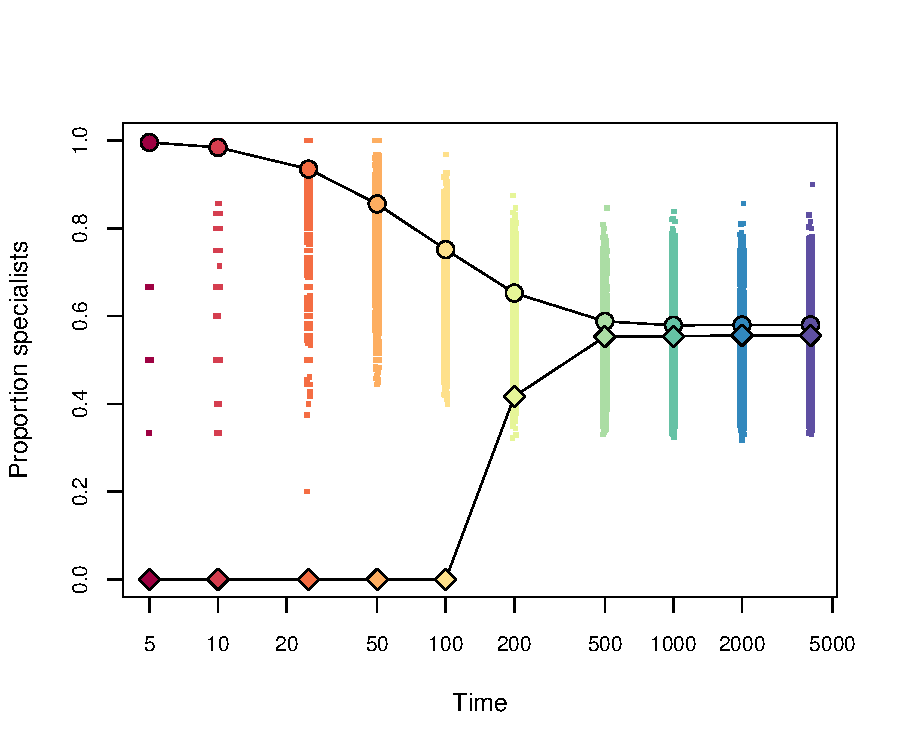
\includegraphics[width=0.5\textwidth]{fig_specialization.pdf}
% \caption{
% The proportion of specialists as a function of assembly time, where a specialist is defined as a species with a generality index $G_i < 1$.
% All measures of $G_i$ are scaled by the average number of links per species $L/S$, and we consider different values of $L/S$ on $G_i$:
% Circles: $G_i^{\rr{all}}$ where $L$ accounts for all links in the food web and $S$ accounts for all species relative to each time interval in the assembly process (averaged across replicates);
% Points: $G_i^{\rr{hetero}}$, where we consider only the links and species richness of heterotrophs, excluding autotrophs (each point shows an individual replicate);
% Diamonds: $G_i^*$, where $L$ and $S$ are measured with respect to the communities at steady state, which is most similar to the measure used to evaluate assembling mangrove food webs (averaged across replicates).
% }
% \label{fig:spec}
% \end{figure}




%Generality
Recent empirical work has suggested that generalist species may dominate early in assembly, whereas specialists colonize after a diverse resource base has accumulated \cite{Piechnik2008,Gravel2011}.
% Here the trophic generality of species $i$ is defined $G_i = k^{\rm in}_i/(L/S)$ where $k^{\rm in}_i$ is the in-degree, or number of resources consumed, by species $i$ \cite{Williams2000}.
Here the trophic generality of species $i$ is defined as $G_i(t) = k_i^{in}(t)/(L^*/S^*)$ \cite{Williams2000}, where $k_i^{in}(t)$ is the number of resource species linked to consumer $i$ at simulation time-step $t$, which is scaled by the steady state link density $L^*/S^*$, as is typically performed in empirical investigations \cite{Piechnik2008}.
Only trophic links between species are considered here, such that we ignore links to the abiotic basal resource in our evaluation of trophic generality.
A species is classified as a generalist if $G_i > 1$ and a specialist if $G_i < 1$.
% In empirical investigations, generality is often scaled to the steady state link density $L^*/S^*$.
If generality is evaluated with respect to the steady state link density, we find that species with many potential trophic interactions realize only a subset of them, thereby functioning as specialists early in the assembly process (Fig.\ \ref{fig:trophic}b).
As the community grows, more potential interactions become realized, and functional specialists become functional generalists.
Moreover, as species assemble, the available niche space expands, and the proportion of potential trophic specialists grows (Fig.\ \ref{fig:trophic}b).
This latter observation confirms expectations from the trophic theory of island biogeography \cite{Gravel2011}, where communities with lower richness (i.e. early assembly) are less likely to support specialist consumers than species-rich communities (late assembly).
% where communities with lower richness (early in assembly) are more likely to support generalist consumers than communities with higher richness (late in assembly). 
At steady state the proportion of functional specialists is ca. 56\%, which is similar to empirical observations of assembling food webs \cite{Piechnik2008}.
%, all measures of $L/S$ are approximately equivalent, and


%trophic levels
%Trophic Levels & degree dists
The dominance of functional specialists following the initial assembly of autotrophs is due to the colonization of lower-trophic consumers with few resources, where the observed trophic level (TL) distribution early in assembly ($t=5$) has an average ${\rm TL}=1.6$.
% Additional consumers arrive in the form of both mixotrophs (consuming the basal resource and one or more autotrophs) and heterotrophs, which establish higher trophic levels.
Four trophic levels are typically established by $t=50$, where colonization is still dominant, and by the time communities reach steady state the interaction networks are characterized by an average ${\rm TL_{max}}$ ($\pm$ standard deviation) $=11 \pm 2.8$ (Fig.\ \ref{fig:trophic}c).
While the maximum trophic level is higher than that measured in most consumer-resource systems \cite{Williams2002}, it is not unreasonable if parasitic interactions (which we do not differentiate from other consumers) are included \cite{Lafferty2006}.
Overall, the most common trophic level among species at steady state is ca. ${\rm TL}=4.75$. %, which is similar to average measures  \cite{Williams2002}.

The distribution of trophic levels changes shape over the course of assembly.
Early in assembly, we observe a skewed pyramidal structure, where most species feed from the base of the food web.
At steady state, we observe that intermediate trophic levels dominate, with frequencies taking on an hourglass structure (purple bars, Fig.\ \ref{fig:trophic}c).
Compellingly, the trophic richness pyramids that we observe at steady state follow closely the hourglass distribution observed for empirical food webs and are less top-heavy than those produced by static food web models \cite{Turney2016}.\\




% We emphasize that these structures are diversity-weighted rather than biomass or abundance-weighted as is often the case \cite{Trebilco2013,Gibert2019}.
% Trophic levels higher than 7 do occur, but are rare.

%Cascading extinctions: Thebault
%Assembly patterns: Barbier
%Origin of ecological structure: Stokstad


%Drossel
% [RELATE TO TROPHIC ASSEMBLY MODELS]\\
%Hourglass food webs are predicted for systems where body size increases with trophic position (marine systems)



% 4) Increased mutualisms => greater nestedness
\vspace{0mm}
\noindent \textbf{Structure and dynamics of mutualisms.}
Nested interactions, where specialist interactions are subsets of generalist interactions, are a distinguishing feature of mutualistic networks \cite{Bascompte2003,Bascompte2006,Guimaraes2006,Araujo2010}.
 % and are defined by asymmetric interactions between species \cite{Bascompte2003,Bascompte2006,Guimaraes2006,Araujo2010}.
Nestedness has been shown to maximize the structural stability of mutualistic networks \cite{Rohr2014}, emerge naturally via adaptive foraging behaviors \cite{Valdovinos2016,Valdovinos2019} and neutral processes \cite{Krishna2008}, and promote the influence of indirect effects in driving coevolutionary dynamics \cite{Guimaraes2017}.
While models and experiments of trophic networks suggest that compartmentalization confers greater stabilizing properties \cite{Stouffer2011,Gilarranz2017}, interaction asymmetry among species may promote nestedness in both trophic \cite{Araujo2010} and mutualistic systems \cite{Pires2011}.
Processes that operate on different temporal and spatial scales may have a significant influence on these observations \cite{Massol2011}.
For example, over evolutionary time, coevolution and speciation may degrade nested structures in favor of modularity \cite{Ponisio2019}, and there is some evidence from Pleistocene food webs that geographic insularity may reinforce this process \cite{Yeakel2013}.

\vspace{0mm}
\begin{figure}[h!]
\centering
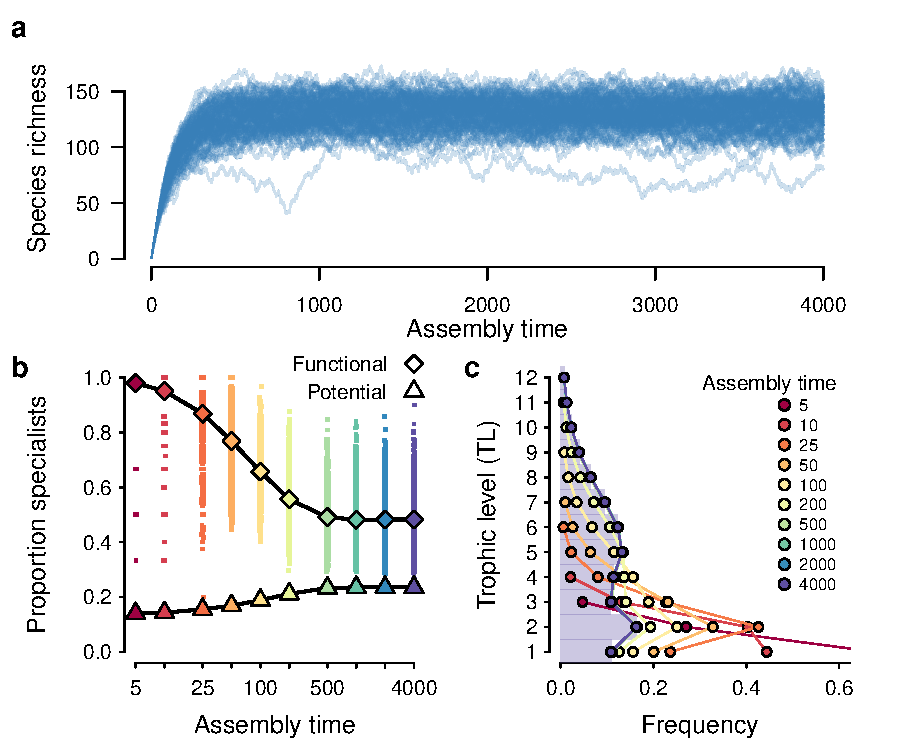
\includegraphics[width=0.5\textwidth]{fig_trophic3.pdf}
\vspace{0mm}
\caption{
Food web structure over the course of assembly.
\textbf{a}, Assembling communities over time from a pool of 200 non-engineering species. 
Steady state species richness is reached by $t=250$.
\textbf{b}, The proportion of specialists as a function of assembly time (iterations), where a specialist is defined as a species with a generality index $G_i < 1$.
All measures of $G_i$ are scaled by the average number of links per species where $L$ and $S$ are measured at steady state.
Diamonds denote expected values for functional (realized) trophic interactions at each point in time, and triangles denote expected values for potential trophic interactions (as if all trophic interactions with all species in the pool were realized), where the expectation is taken across replicates. Individual replicate results are shown for functional trophic interactions (small points).
\textbf{c}, The frequency distribution of trophic levels as a function of assembly time (iterations). 
Autotrophs occupy ${\rm TL}=1$.
Measures were evaluated across $10^4$ replicates; see Methods for parameter values.
\vspace{0mm}
}
\label{fig:trophic}
\end{figure}


Does the assembly of ecological networks favor nestedness when mutualistic interactions are frequent?
In the absence of mutualisms, the trade-offs in our model preclude high levels of nestedness because we assume that generalists are at a competitive disadvantage when they share the same resources with a specialist consumer.
Yet we find that as we increase the frequency of service interactions (holding constant trophic interaction frequency; see Supplementary Appendix 2), the assembled community at steady state becomes more nested (Fig.\ \ref{fig:nest}a).
More service interactions increase a species' competition strength, lowering its primary extinction risk.
Participation in a mutualism thus delivers a fitness advantage to the species receiving the service, compensating for the lower competitive strength of generalists and allowing generalists to share subsets of resources with specialists, which promotes nestedness.
However increases in mutualisms also increase inter-species dependencies, which raises the potential risk associated with losing mutualistic partners \cite{Bond1994,Colwell2012}. % and its secondary extinction risk
% Indeed, the balance that mutualists must maintain with their partners may have large implications for the future of global biodiversity \cite{Dunn2009}.
While this shifting landscape of extinction risks lowers the steady state species richness of highly mutualistic communities, we do not observe a direct relationship between nestedness and richness (Fig.\ \ref{fig:nestsize}).

When we examine the dynamics of the community as a function of service interaction frequency, we observe that mutualistic interactions have different effects on primary versus secondary extinction rates.
Because service dependencies bolster the competitive strength of otherwise susceptible species such as trophic generalists and species with multiple predators, the rate of primary extinctions is lowered, though this effect is weak (Fig.\ \ref{fig:nest}b).
However, because mutualisms build rigid dependencies between species, more service interactions result in higher frequencies of secondary extinctions (Fig.\ \ref{fig:nest}c). 
In communities with many mutualistic interactions, this combined influence yields extinctions that are less likely to occur, but lead to larger cascades when they do.

An increased rate of secondary extinctions means that the network is less robust to perturbation, which may impact community turnover, or persistence.
If we measure persistence in terms of the proportion of time species are established in the community, we find that higher frequencies of service interactions lower average persistence (increased species turnover; Fig.\ \ref{fig:nest}d).
Analysis of species-specific interactions reveals that it is the species that require more services that have lower persistence (Fig.\ \ref{fig:degree}).
% Persistence as measured as the percent simulation time the community is occupied by a given species, averaged across all species that successfully colonize.
% At the community-scale, lower average persistence implies greater species turnover.
Observations of empirical systems appear to support model predictions.
For example, assembling plant-pollinator systems have demonstrated high rates of species and interaction turnover, both during the assembly process and at the steady state \cite{DiazCastelazo2013}. %\cite{Ponisio2017}


\begin{figure}[h!]
\centering
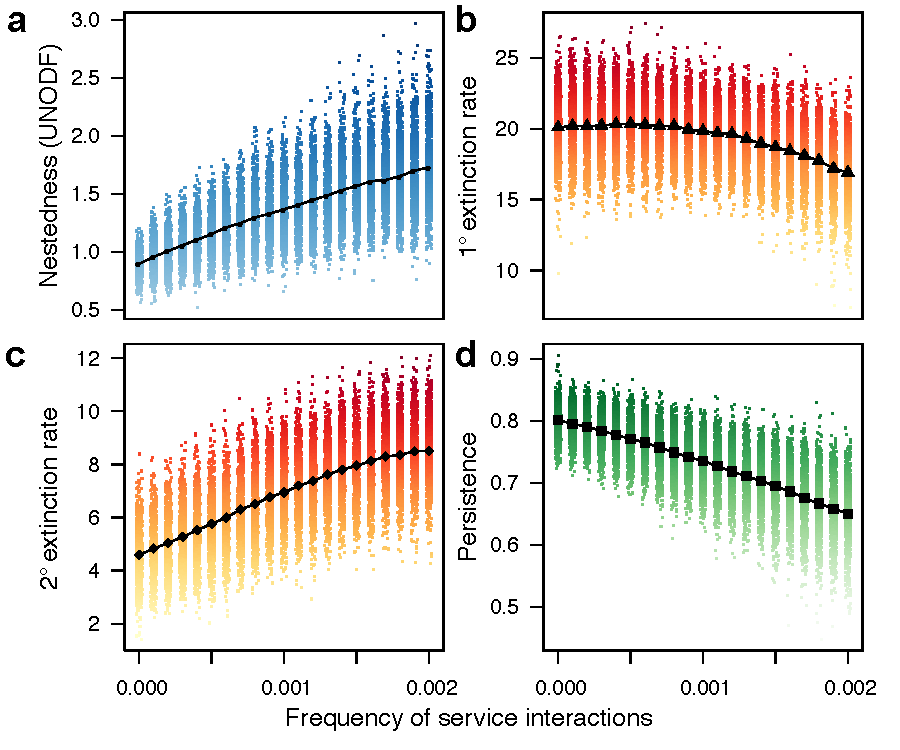
\includegraphics[width=0.5\textwidth]{fig_nested4.pdf}
\vspace{-6mm}
\caption{
Community structure and stability as a function of the frequency of service interactions.
\textbf{a}, Structural nestedness of communities, measured as UNODF (Unipartite Nestedness based on Overlap and Decreasing Fill) \cite{Cantor2017}.
The value reported is the mean value taken across the rows and columns of the adjacency matrix accounting for both trophic and service interactions.
% Inset: A trophic and mutualistic nested motif for resource species 1, 2 and consumer species 3, 4.
% Whether the interactions are trophic or mutualistic impacts the susceptibility of each species to primary extinctions (based on differences in competitive strength $\sigma_i$) and secondary extinctions (which result from lost dependencies associated with primary extinctions).
\textbf{b}, Mean rate of primary extinction  (where primary extinctions occur from competitive exclusion of consumers over shared resources) and \textbf{c}, secondary extinction (which cascade from primary extinctions) as a function of service interaction frequency.
\textbf{d}, Species persistence as a function of service interaction frequency.
Primary and secondary extinction rates were evaluated at the community level, whereas persistence was determined for each species and averaged across the community.
Measures were evaluated for $10^4$ replicates; see Methods and Supplementary Appendix 2 for parameter values.
\vspace{-6mm}
}
\label{fig:nest}
\end{figure}


% An important condition of our model is that we assume that all service interactions are obligate (see Methods), which is expected to heighten the influence of secondary extinctions.
We emphasize that we have restricted ourselves to examining the effects of obligate mutualisms, although the importance of non-obligate mutualisms has long been recognized \cite{RamosJiliberto2012,Vieira2015,Valdovinos2016,Ponisio2017,Valdovinos2019}.
% Because including these
% While the inclusion of non-obligate mutualists will lower the likelihood of cascading effects in systems with higher frequencies of service interactions, the loss of obligate mutualistic partners will have larger dynamic consequences than the loss of more flexible non-obligate mutualistic partners.
We expect that the increased rate of secondary extinctions attributable to the loss of obligate mutualistic partners to have greater impact on system stability than the potential loss of non-obligate mutualistic partners.
As such, we do not expect inclusion of non-obligate mutualisms to alter the qualitative nature of our findings.\\
% In future efforts, we aim to explore how the combination of obligate and non-obligate mutualisms impact community dynamics.
% In future efforts, we aim to explore the effects of both obligate and non-obligate mutualistic interactions on community assembly.\\
%What is the CV of mutualistic trajectories?




\vspace{0mm}
\noindent \textbf{Assembly with ecosystem engineering.}
%Theory
The concept of ecosystem engineering, or more generally niche construction, has both encouraged an extended evolutionary synthesis \cite{Laland2015} while also garnering considerable controversy \cite{Gupta2017,Feldman2017}.
Models that explore the effects of ecosystem engineering are relatively few, but have covered important ground \cite{Hastings2007,OdlingSmee2013}.
For example, engineering has been shown to promote invasion \cite{Cuddington2004}, alter primary productivity \cite{Wright2004}, and change the selective environment over eco-evolutionary timescales \cite{Kylafis2008,Krakauer2009} which can lead to unexpected outcomes such as the fixation of deleterious alleles \cite{Laland1999}.
% Initial work focused on understanding how habitat modification might impact the persistence of engineering species \cite{Gurney1996}, while more recent efforts have shown that engineering can promote invasion \cite{Cuddington2004} and impact primary productivity \cite{Wright2004}.
% On eco-evolutionary timescales, ecosystem engineering can alter the selective environment \cite{Krakauer2009,OdlingSmee2013} and ultimately lead to unexpected outcomes such as the fixation of deleterious alleles \cite{Laland1999}.
% On macroevolutionary timescales, there is considerable interest in understanding the role of innovation on diversification and extinction rates within and among clades \cite{Marshall2016}.
% While such innovation generally pertains to the appearance of morphological traits, environmental modifications that result from evolutionary innovations can sometimes be wide-ranging, such as the planetary-scale consequences following the evolution of multicellular cyanobacteria \cite{Schirrmeister2013}.
On smaller scales, microbiota construct shared metabolitic resources that have a significant influence on microbial communities \cite{Kallus2017}, the dynamics of which may even serve as the missing ingredient stabilizing some complex ecological systems \cite{Butler2018}.
The soil is one place where these macro- and microbiotic systems intersect \cite{Amundson2015}.
Many microbes and detritivores transform and deliver organic matter into the macrobiotic food web, themselves hosting a complex network of trophic and service dependencies between species and abiotic entities \cite{Gutierrez2006,Jouquet2006}.
%DG: a good case that I completely missed in the first version but that is common, fundamental and relatevely well studied is the soil food web. Microbes and detritivores usually transform the organic matter, changing it's quality and physical state as we move through the processing chain. I've played with such models and a distinct feature they have is the frequence of donor-controlled types of interactions. The transformed organic matter is simply a byproduct of consumption, produced at a rate determined by the provider, not the one benefiting from it. It generates a lot of +,0 interactions that are currently understudied, but also prevalent here in the model. The parallel may further strengthen the paper and also open it to a wider audience. 


We next explore the effects of ecosystem engineering by allowing species to produce abiotic modifiers as additional nodes in the ecological network (Fig.\ \ref{fig:model}).
These modifier nodes produced by engineers can serve to fulfill resource or service requirements for other species.
The parameter $\eta$ defines the mean number of modifiers produced per species in the pool, drawn from a Poisson distribution (see Methods and Supplementary Appendix 1 for details).
If a species makes $\geq 1$ modifier, we label it an engineer.
As the mean number of modifiers/species $\eta$ increases, both the number of engineers in the pool as well as the number of modifiers made per engineer increases.
As detailed in Supplementary Appendix 1, multiple engineers can make the same modifier, such that engineering redundancies are introduced when $\eta$ is large.
When an engineer colonizes the community, so do its modifiers, which other species in the system may interact with.
When engineers are lost, their modifiers will also be lost, though can linger in the community for a period of time inversely proportional to the density of disconnected modifiers in the community (see Supplementary Appendix 1).
% There are two characteristics of engineering that have particular relevance for community assembly: modifiers can linger in the community even after the species that produce them have been excluded, and more than one engineer can produce the same modifier such that engineering redundancies increase with $\eta$.




%Engineering can produce positive feedback dynamics on engineers
%Positive feedback over evolutionary time => speciation/radiation
%Lead to engineering redundancies
%This may be rare as Lawton suggests, but appears to be quite common in the microbial world.
%In microbiomes, horizontal gene transfer can produce redundant engineering without radiations

%Lawton 1994: there may be sometimes redundancy in ecosystem engineers... (uses beaver to suggest that there is not)

%negative (introduces dependencies) then positive (introduces redundancies)
While the inclusion of engineering does not significantly impact the structure of species-species interactions within assembling food webs (see Supplementary Appendix 4 and Fig.\ \ref{fig:trophiceng}), it does have significant consequences for community stability.
Importantly, these effects also are sensitive to the frequency of service interactions within the community, and we find that their combined influence can be complex.

% Increasing engineering has different effects on primary versus secondary extinctions.
As the number of engineers increases, mean rates of primary extinction are first elevated and then decline (Fig.\ \ref{fig:engineers}a).
At the same time, the mean rates of secondary extinction systematically decline and persistence systematically increases (Fig.\ \ref{fig:engineers}b-c).
When engineered modifiers are rare ($0 < \eta \leq 0.5$), higher rates of primary extinction coupled with lower rates of secondary extinction mean that extinctions are common, but of limited magnitude such that disturbances are compartmentalized.
As modifiers become more common both primary and secondary extinction rates decline, which corresponds to increased persistence.
We suggest two mechanisms that may produce the observed results.
First, when engineers and modifiers are present but rare, they provide additional resources for consumers.
This stabilization of consumers ultimately results in increased vulnerability of prey, such that the cumulative effect is increased competitive exclusion of prey and higher rates of primary extinction (Fig.\ \ref{fig:engineers}a).
Second, when engineers and their modifiers are common ($\eta > 0.5$) the available niche space expands, lowering competitive overlap and suppressing both primary and secondary extinctions.
Notably the presence of even a small number of engineers serves to limit the magnitude of secondary extinction cascades.
Assessment of species persistence as a function of trophic in-degree (number of resources) and out-degree (number of consumers) generally supports this proposed dynamic (Fig.\ \ref{fig:indeng}).

% This nonlinear effect of engineering on rates of primary extinction results from two competing forces.
% The first force is observed when engineers and their modifiers are rare ($0 < \eta \leq 0.5$).
% Increased production of abiotic modifiers supplies consumers with additional resources, limiting secondary extinctions and promoting persistence (Fig.\ \ref{fig:engineers}B,~C).


%Mutualisms + Engineering
Increasing the frequency of service interactions promotes service interactions between species and engineered modifiers (Fig.\ \ref{fig:model}).
A topical example of the latter is the habitat provided to invertebrates by the recently discovered rock-boring teredinid shipworm (\emph{Lithoredo abatanica}) \cite{Shipway2019}.
Here, freshwater invertebrates are serviced by the habitat modifications engineered by the shipworm, linking species indirectly via an abiotic effect (in our framework via a modifier node).
As the frequency of service interactions increases, the negative effects associated with rare engineers is diminished (Fig.\ \ref{fig:engineers}a).
Increasing service interactions both elevates the competitive strength of species receiving services (from species and/or modifiers), while creating more interdependencies between and among species.
% Species that serve as resources to many consumers are less competitive due to increased vulnerability.
As trophic interactions are replaced by service interactions, previously vulnerable species gain a competitive foothold and persist, lowering rates of primary extinctions (Fig.\ \ref{fig:engineers}a). %, particularly in systems where consumers are facilitated by a small number of engineers
The cost of these added services to the community is an increased rate of secondary extinctions (Fig.\ \ref{fig:engineers}b) and higher species turnover (Fig.\ \ref{fig:engineers}c), such that extinctions are less common but lead to larger cascades.
% Low rates of primary extinction coupled with high rates of secondary extinction mean that extinctions are less common but lead to larger cascades.
% Importantly, these changes are not due to fluctuations in steady state community richness, which remains relatively constant across the parameter space that we examine (Fig.\ \ref{fig:steadystate}A).

% Together, these results point to an important tradeoff originating from the effects of engineering.
% When engineering and servive interactions are rare, extinction rates are higher, but have smaller consequences; as mutualisms become more common, extinction rates are lower, but have larger consequences.


% Ecosystem engineers can be stabilizing agents in communities if they primarily serve to provide additional resources to non-specialist consumers.
% However if species' presence in the community require the effects induced by engineers, their cumulative influence can be destabilizing.
% Whether engineers are stabilizing or destabilizing is thus largely determined by the flexibility of inter-dependencies connecting species in a community.
% Redundancy in engineered effects both lowers extinction rates while increasing the time that individual species are present within the assembling community.

\vspace{0mm}
\begin{figure}[h!]
\centering
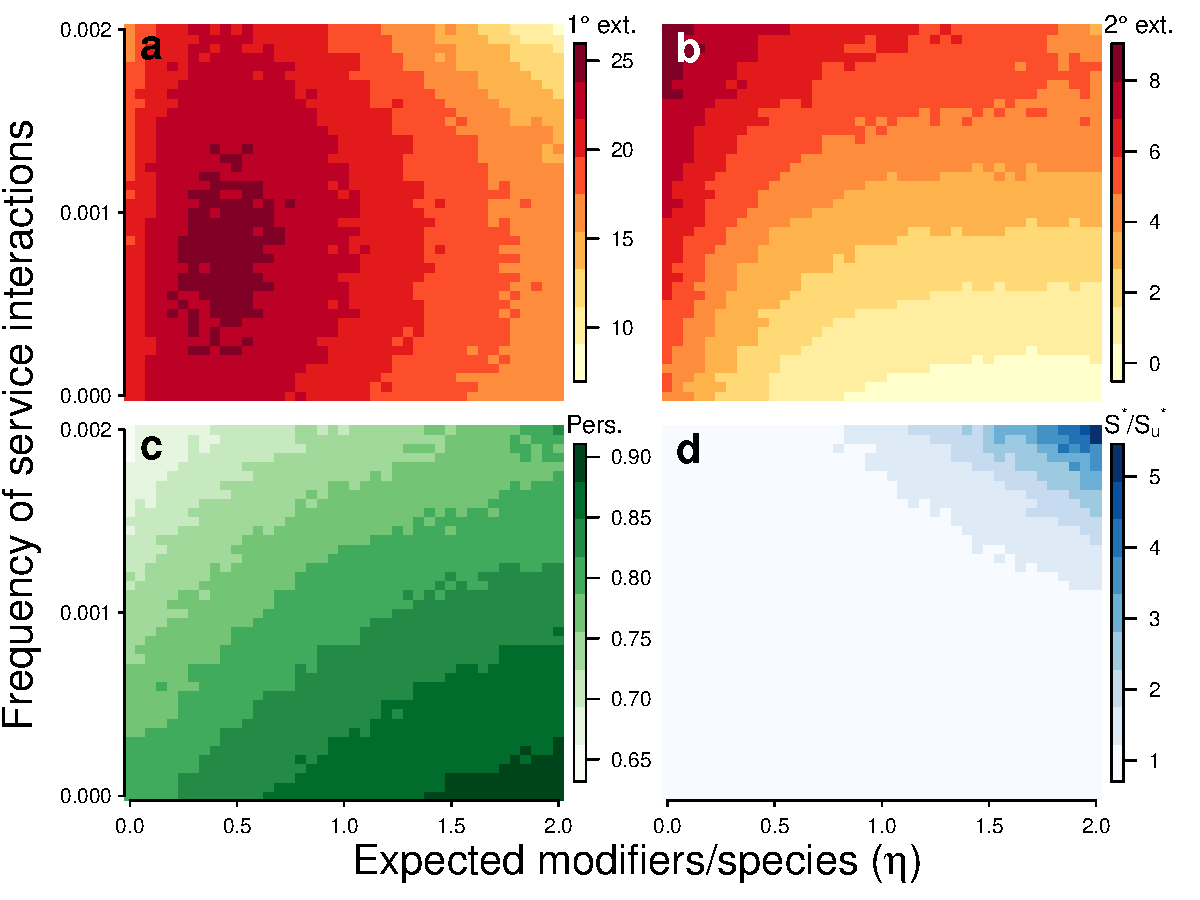
\includegraphics[width=0.5\textwidth]{fig_engineers6.pdf}
\vspace{-8mm}
\caption{
Community stability as a function of the frequency of service interactions and modifiers per species.
\textbf{a}, Mean rates of primary extinction, where primary extinctions occur from competitive exclusion of consumers over shared resources.
\textbf{b}, Mean rates of secondary extinction, which cascade from primary extinctions.
\textbf{c}, Mean species persistence.
\textbf{d}, The ratio $S^*/S^*_{\rm u}$, where $S^*_{\rm u}$ denotes steady states for systems where all engineered modifiers are unique to each engineer, and $S^*$ denote steady states for systems with redundant engineering. Higher values of $S^*/S^*_{\rm u}$ mean that systems with redundant engineers have higher richness at the steady state than those without redundancies.
Primary and secondary extinction rates were evaluated at the community level, whereas persistence was determined for each species and averaged across the community.
Each measure reports the expectation taken across $50$ replicates.
See Methods and Supplementary Appendix 2 for parameter values.
\vspace{0mm}
}
\label{fig:engineers}
\end{figure}



While the importance of engineering timescales has been emphasized previously \cite{Hastings2007}, redundant engineering has been assumed to be unimportant \cite{Lawton1994}.
We argue that redundancy may be an important component of highly engineered systems, and particularly relevant when the effects of engineers increase their own fitness \cite{Cuddington2004} as is generally assumed to be the case with niche construction \cite{Krakauer2009}.
If ecosystem engineering also includes, for example, biogeochemical processes such as nitrogen-fixing among plants and mycorrhizal fungi, redundancy may be perceived as the rule rather than the exception.
% exists a positive feedback between the effects of engineers on their fitness \cite{Cuddington2004}.
Moreover, the vast majority of contemporary ecosystem engineering case studies focus on single taxa, such that redundant engineers appear rare \cite{Lawton1994}.
If we consider longer timescales, diversification of engineering clades may promote redundancy, and in some cases this may feed back to accelerate diversification \cite{OdlingSmee2013b}.
Such positive feedback mechanisms likely facilitated the global changes induced by cyanobacteria in the Proterozoic \cite{Erwin2008,Schirrmeister2013} among other large-scale engineering events in the history of life \cite{Erwin2008}.
Engineering redundancies are likely important on shorter timescales as well.
For example, diverse sessile epifauna on shelled gravels in shallow marine environments are facilitated by the engineering of their ancestors, such that the engineered effects of the clade determine the future fitness of descendants \cite{Kidwell1986}.
In the microbiome, redundant engineering may be very common due to the influence of horizontal gene transfer in structuring metabolite production \cite{Polz2013}.
In these systems, redundancy in the production of shared metabolitic resources may play a key role in community structure and dynamics \cite{Kallus2017,Butler2018}.




% %Role of Redundancy
When there are few engineers, each modifier in the community tends to be unique to a particular engineering species.
Engineering redundancies increase linearly with $\eta$ (Supplementary Appendix 1; Fig.\ \ref{fig:redundancy}), such that the loss of an engineer will not necessarily lead to the loss of engineered modifiers. % if alternative engineers persist.
We examine the effects of this redundancy by comparing our results to those produced by the same model, but where each modifier is uniquely produced by a single species.
Surprisingly, the lack of engineering redundancies does not alter the general relationship between engineering and measures of community stability (Fig.\ \ref{fig:unique}).
However we find that redundancies play a central role in maintaining species diversity.
When engineering redundancies are allowed, steady state community richness $S^*$ does not vary considerably with increasing service interactions and engineering (Fig.\ \ref{fig:steadystate}a).
In contrast, when redundant engineering is not allowed, steady state community richness $S^*_u$ declines sharply (Figs. \ref{fig:engineers}d, \ref{fig:steadystate}b).

Communities lacking redundant engineering have lower species richness because species' trophic and service dependencies are unlikely to be fulfilled within a given assemblage (Fig.\ \ref{fig:steadystate}c,d).
Colonization occurs only when trophic and service dependencies are fulfilled.
A species requiring multiple engineered modifiers, each uniquely produced, means that each required entity must precede colonization.
This magnifies the role of priority effects in constraining assembly order \cite{Fukami2015}, precluding many species from colonizing.
In contrast, redundant engineering increases the temporal stability of species' niches while minimizing priority effects by allowing multiple engineers to fulfill the dependencies of a particular species.
Our results thus suggest that redundant engineers may play important roles in assembling ecosystems by lowering the barriers to colonization, promoting community diversity.

%Closing
% \rev{We have shown that the dynamics of assembly driven by multitype interactions can produce model communities with realistic structures and dynamics.
% Moreover, the inclusion of ecosystem engineering by way of modifier nodes reveals that low levels of engineering may be expected to produce higher rates of extinction while limiting the size of extinction cascades, and that engineering redundancy -- whether it is common or rare -- may have considerable dynamical implications.}
We have shown that simple process-based rules governing the assembly of species with multitype interactions can produce communities with realistic structures and dynamics.
Moreover, the inclusion of ecosystem engineering by way of modifier nodes reveals that low levels of engineering may be expected to produce higher rates of extinction while limiting the size of extinction cascades, and that engineering redundancy -- whether it is common or rare -- serves to promote colonization and by extension diversity.
We suggest that including the effects of engineers, either explicitly as we have done here, or otherwise, is vital for understanding the inter-dependencies that define ecological systems.
As past ecosystems have fundamentally altered the landscape on which contemporary communities interact, future ecosystems will be defined by the influence of engineering today.
Given the rate and magnitude with which humans are currently engineering environments \cite{Corlett2015}, understanding the role of ecosystem engineers is thus tantamount to understanding our own effects on the assembly of natural communities.\\






% \begin{matmethods}
\vspace{-2mm}
\noindent \textbf{Methods}\\
  \footnotesize{
  % \noindent \textbf{The ENIgMa Model}\\
  We model an ecological system with a network where nodes represent `ecological entities' such as populations of species and or the presence of abiotic modifiers affecting species.
   % and links represent interactions between them.
  Following Pilai et al. \cite{Pillai2011}, we do not track the abundances of entities but track only their presence or absence (see also Refs. \cite{Luh1993,Campbell2011}).
  The links of the network represent interactions between pairs of entities (x,y).
  We distinguish three types of such interactions: x eats y, x needs y to be present, x makes modifier y.

  The assembly process entails two steps: first a source pool of species is created, followed by colonization/extinction into/from a local community.
  The model is initialized by creating $S$ species and $M = \eta S$ modifiers, such that $N=S+M$ is the expected total number of entities (before considering engineering redundancies) and $\eta$ is the expected number of modifiers made per species in the community, where the expectation is taken across independent replicates.
  For each pair of species (x,y) there is a probability $p_e$ that x eats y and probability $p_n$ that x needs y.
  For each pair of species x and modifier m, there is a probability $q_e$ that species x eats modifier m and a probability $q_n$ that species x needs modifier m.
  Throughout we assume that $p_e = q_e$ and $p_n = q_n$ for simplicity.
  Each species $i$ makes a number of modifiers $M_i \sim \rr{Poiss}(\eta)$. %where $\eta$ is the mean number of modifiers made per species.
  If engineering redundancies are allowed, once the number of modifiers per species is determined each modifier is assigned to a species independently to match its assigned number of modifiers.
  This means that multiple species may make the same modifier, and that there may be some modifiers that are not assigned to any species, which are eliminated from the pool.
  Accounting for engineering redundancies, the number of modifiers in the pool becomes $M^\prime = \eta S (\rr{e}-1)/\rr{e}$ where $\rr{e}$ is Euler's number.
  If engineering redundancies are not allowed, each modifier is made by a single engineer and $M^\prime = M$.
  
  In addition to interactions with ecosystem entities, there can be interactions with a basal resource, which is always present.
  The first species always eats this resource, such that there is always a primary producer in the pool.
  Other species eat the basal resource with probability $p_e$.
  Species with zero assigned trophic interactions are assumed to be primary producers.
  See Supplementary Appendix 1 for additional details on defining the source pool.

  We then consider the assembly of a community which at any time will contain a subset of entities in the pool and always the basal resource.
  In time, the entities in the community are updated following a set of rules.
  A species from the pool can colonize the community if the following conditions are met:
  1) all entities that a species needs are present in the community, and
  2) at least one entity that a species eats is present in the community.
  If a colonization event is possible, it occurs stochastically in time with rate $r_\rr{c}$.

  An established species is at risk of extinction if it is not the strongest competitor at least one of its resources that it eats.
  We compute the competitive strength of species $i$ as
  \begin{equation}
    \sigma_i = c_\rr{n} n_i - c_\rr{e} e_i - c_\rr{v} v_i,
  \end{equation}
  where $n_i$ is the number of entities that species $i$ needs, $e_i$ is the number of entities from the pool that species $i$ can eat, and $v_i$ is the number of species in the community that eat species $i$.
  This captures the ecological intuition that mutualisms provide a fitness benefit \cite{Bronstein1994}, specialists are stronger competitors than generalists \cite{Futuyma1988}, and many predators entail an energetic cost \cite{Brown1994}.
  The coefficients $c_\rr{n},~c_\rr{e},~c_\rr{v}$ describe the relative effects of these contributions to competition strength.
  In the following, we use the relationship $c_\rr{n} > c_\rr{e} > c_\rr{v}$, such that the competitive benefit of adding an additional mutualism is greater than the detriment incurred by adding another resource or predator.
  % In the following, we use the values $c_\rr{n} = \pi,~c_\rr{e}=\sqrt{2},~c_\rr{v}=1$, such that the competitive benefit of adding an additional mutualism is greater than the detriment incurred by adding another prey or predator.
  A species at risk of extinction leaves the community stochastically in time at rate $r_e$.

  A modifier is present in the community whenever at least one species that makes the modifier is present.
  If a species that makes a modifier colonizes a community, the modifier is introduced as well, however modifiers may persist for some time after the last species that makes the modifier goes extinct.
  Any modifier that has lost all of its makers disappears stochastically in time at rate $r_m$.

  The model described here can be simulated efficiently with an event-driven simulation utilizing a Gillespie algorithm.
  In these types of simulations, one computes the rates $r_j$ of all possible events $j$ in a given step.
  One then selects the time at which the next event happens by drawing a random number from an exponential distribution with mean $1/\sum_j{r_j}$.
  At this time, an event occurs that is randomly selected from the set of possible events such that the probability of event $a$ is $r_a/\sum_j{r_j}$.
  The effect of the event is then realized and the list of possible events is updated for the next step.
  This algorithm is known to offer a much better approximation to the true stochastic continuous time process than a simulation in discrete time steps, while providing a much higher numerical efficiency \cite{Gillespie1977}.
  Simulations described in the main text have default parameterizations of $S=200$, $p_e=0.01$, $c_{\rm n} = \pi$, $c_{\rm e} = \sqrt{2}$, $c_{\rm v} = 1$, and $4000$ iterations.
  Replicates are defined as the independent assembly of independently drawn source pools with a given parameterization.}

\vspace{2mm}
\noindent \textbf{Data availability}\\
  \footnotesize{
  The study is theoretical; no new empirical data were generated.
  }\\ \\
\noindent \textbf{Code availability}\\
  \footnotesize{
  The simulation code supporting this work is available for download from https://github.com/jdyeakel/Lego.
  }\\

%\putbib[aabib]
% \begin{thebibliography}{10}
% \expandafter\ifx\csname url\endcsname\relax
%   \def\url#1{\texttt{#1}}\fi
% \expandafter\ifx\csname urlprefix\endcsname\relax\def\urlprefix{URL }\fi
% \providecommand{\bibinfo}[2]{#2}
% \providecommand{\eprint}[2][]{\url{#2}}
% 
% \bibitem{Paine1966}
% \bibinfo{author}{Paine, R.~T.}
% \newblock \bibinfo{title}{Food web complexity and species diversity}.
% \newblock \emph{\bibinfo{journal}{Am. Nat.}} \textbf{\bibinfo{volume}{100}},
%   \bibinfo{pages}{65--75} (\bibinfo{year}{1966}).
% 
% \bibitem{Dunne2002}
% \bibinfo{author}{Dunne, J.~A.}, \bibinfo{author}{Williams, R.~J.} \&
%   \bibinfo{author}{Martinez, N.~D.}
% \newblock \bibinfo{title}{Food-web structure and network theory: the role of
%   connectance and size}.
% \newblock \emph{\bibinfo{journal}{Proc. Natl. Acad. Sci. USA}}
%   \textbf{\bibinfo{volume}{99}}, \bibinfo{pages}{12917--12922}
%   (\bibinfo{year}{2002}).
% 
% \bibitem{Pascual2006}
% \bibinfo{author}{Pascual, M.} \& \bibinfo{author}{Dunne, J.}
% \newblock \emph{\bibinfo{title}{Ecological Networks: Linking Structure to
%   Dynamics in Food Webs}} (\bibinfo{publisher}{Oxford University Press},
%   \bibinfo{address}{Oxford, UK}, \bibinfo{year}{2006}).
% 
% \bibitem{Bascompte2013}
% \bibinfo{author}{Bascompte, J.} \& \bibinfo{author}{Jordano, P.}
% \newblock \emph{\bibinfo{title}{Mutualistic Networks}}.
% \newblock Monographs in Population Biology (\bibinfo{publisher}{Princeton
%   University Press}, \bibinfo{address}{Princeton, NJ}, \bibinfo{year}{2013}).
% 
% \bibitem{May1972}
% \bibinfo{author}{May, R.~M.}
% \newblock \bibinfo{title}{{Will a large complex system be stable?}}
% \newblock \emph{\bibinfo{journal}{Nature}} \textbf{\bibinfo{volume}{238}},
%   \bibinfo{pages}{413--414} (\bibinfo{year}{1972}).
% 
% \bibitem{Gross2009}
% \bibinfo{author}{Gross, T.}, \bibinfo{author}{Levin, S.~A.} \&
%   \bibinfo{author}{Dieckmann, U.}
% \newblock \bibinfo{title}{Generalized models reveal stabilizing factors in food
%   webs}.
% \newblock \emph{\bibinfo{journal}{Science}} \textbf{\bibinfo{volume}{325}},
%   \bibinfo{pages}{747--750} (\bibinfo{year}{2009}).
% 
% \bibitem{Allesina2012}
% \bibinfo{author}{Allesina, S.} \& \bibinfo{author}{Tang, S.}
% \newblock \bibinfo{title}{{Stability criteria for complex ecosystems}}.
% \newblock \emph{\bibinfo{journal}{Nature}} \textbf{\bibinfo{volume}{483}},
%   \bibinfo{pages}{205--208} (\bibinfo{year}{2012}).
% 
% \bibitem{Montoya2003}
% \bibinfo{author}{Montoya, J.~M.} \& \bibinfo{author}{Sol{\'e}, R.~V.}
% \newblock \bibinfo{title}{{Topological properties of food webs: from real data
%   to community assembly models}}.
% \newblock \emph{\bibinfo{journal}{Oikos}} \textbf{\bibinfo{volume}{102}},
%   \bibinfo{pages}{614--622} (\bibinfo{year}{2003}).
% 
% \bibitem{Bascompte2009}
% \bibinfo{author}{Bascompte, J.} \& \bibinfo{author}{Stouffer, D.}
% \newblock \bibinfo{title}{{The assembly and disassembly of ecological
%   networks}}.
% \newblock \emph{\bibinfo{journal}{Philos. T. Roy. Soc. B}}
%   \textbf{\bibinfo{volume}{364}}, \bibinfo{pages}{1781} (\bibinfo{year}{2009}).
% 
% \bibitem{Hubbell2001}
% \bibinfo{author}{Hubbell, S.}
% \newblock \emph{\bibinfo{title}{{The unified neutral theory of biodiversity and
%   biogeography}}} (\bibinfo{publisher}{Princeton Univ Press},
%   \bibinfo{address}{Princeton, USA}, \bibinfo{year}{2001}).
% 
% \bibitem{Tilman2004}
% \bibinfo{author}{Tilman, D.}
% \newblock \bibinfo{title}{Niche tradeoffs, neutrality, and community structure:
%   a stochastic theory of resource competition, invasion, and community
%   assembly}.
% \newblock \emph{\bibinfo{journal}{Proc. Natl. Acad. Sci. USA}}
%   \textbf{\bibinfo{volume}{101}}, \bibinfo{pages}{10854--10861}
%   (\bibinfo{year}{2004}).
% 
% \bibitem{Fukami2015}
% \bibinfo{author}{Fukami, T.}
% \newblock \bibinfo{title}{{Historical Contingency in Community Assembly:
%   Integrating Niches, Species Pools, and Priority Effects}}.
% \newblock \emph{\bibinfo{journal}{Annu. Rev. Ecol. Evol. Syst.}}
%   \textbf{\bibinfo{volume}{46}}, \bibinfo{pages}{1--23} (\bibinfo{year}{2015}).
% 
% \bibitem{Kraft2008}
% \bibinfo{author}{Kraft, N. J.~B.}, \bibinfo{author}{Valencia, R.} \&
%   \bibinfo{author}{Ackerly, D.~D.}
% \newblock \bibinfo{title}{{Functional Traits and Niche-Based Tree Community
%   Assembly in an Amazonian Forest}}.
% \newblock \emph{\bibinfo{journal}{Science}} \textbf{\bibinfo{volume}{322}},
%   \bibinfo{pages}{580--582} (\bibinfo{year}{2008}).
% 
% \bibitem{ODwyer2009}
% \bibinfo{author}{O'Dwyer, J.~P.}, \bibinfo{author}{Lake, J.},
%   \bibinfo{author}{Ostling, A.}, \bibinfo{author}{Savage, V.~M.} \&
%   \bibinfo{author}{Green, J.}
% \newblock \bibinfo{title}{{An integrative framework for stochastic,
%   size-structured community assembly}}.
% \newblock \emph{\bibinfo{journal}{Proc. Natl. Acad. Sci. USA}}
%   \textbf{\bibinfo{volume}{106}}, \bibinfo{pages}{6170} (\bibinfo{year}{2009}).
% 
% \bibitem{Brown2002}
% \bibinfo{author}{Brown, J.~H.}, \bibinfo{author}{Kelt, D.~A.} \&
%   \bibinfo{author}{Fox, B.~J.}
% \newblock \bibinfo{title}{{Assembly Rules and Competition in Desert Rodents}}.
% \newblock \emph{\bibinfo{journal}{Am. Nat.}} \textbf{\bibinfo{volume}{160}},
%   \bibinfo{pages}{815--818} (\bibinfo{year}{2002}).
% 
% \bibitem{Piechnik2008}
% \bibinfo{author}{Piechnik, D.~A.}, \bibinfo{author}{Lawler, S.~P.} \&
%   \bibinfo{author}{Martinez, N.~D.}
% \newblock \bibinfo{title}{{Food-web assembly during a classic biogeographic
%   study: species' {\textquotedblleft}trophic breadth{\textquotedblright}
%   corresponds to colonization order}}.
% \newblock \emph{\bibinfo{journal}{Oikos}} \textbf{\bibinfo{volume}{117}},
%   \bibinfo{pages}{665--674} (\bibinfo{year}{2008}).
% 
% \bibitem{Fahimipour2014}
% \bibinfo{author}{Fahimipour, A.~K.} \& \bibinfo{author}{Hein, A.~M.}
% \newblock \bibinfo{title}{{The dynamics of assembling food webs}}.
% \newblock \emph{\bibinfo{journal}{Ecol. Lett.}} \textbf{\bibinfo{volume}{17}},
%   \bibinfo{pages}{606--613} (\bibinfo{year}{2014}).
% 
% \bibitem{Barbier2018}
% \bibinfo{author}{Barbier, M.}, \bibinfo{author}{Arnoldi, J.-F.},
%   \bibinfo{author}{Bunin, G.} \& \bibinfo{author}{Loreau, M.}
% \newblock \bibinfo{title}{{Generic assembly patterns in complex ecological
%   communities}}.
% \newblock \emph{\bibinfo{journal}{Proc. Natl. Acad. Sci. USA}}
%   \textbf{\bibinfo{volume}{115}}, \bibinfo{pages}{2156--2161}
%   (\bibinfo{year}{2018}).
% 
% \bibitem{Campbell2011}
% \bibinfo{author}{Campbell, C.}, \bibinfo{author}{Yang, S.},
%   \bibinfo{author}{Albert, R.} \& \bibinfo{author}{Shea, K.}
% \newblock \bibinfo{title}{{A network model for plant-pollinator community
%   assembly}}.
% \newblock \emph{\bibinfo{journal}{Proc. Natl. Acad. Sci. USA}}
%   \textbf{\bibinfo{volume}{108}}, \bibinfo{pages}{197--202}
%   (\bibinfo{year}{2011}).
% 
% \bibitem{Luh1993}
% \bibinfo{author}{Hang-Kwang, L.} \& \bibinfo{author}{Pimm, S.~L.}
% \newblock \bibinfo{title}{The assembly of ecological communities: A minimalist
%   approach}.
% \newblock \emph{\bibinfo{journal}{J. Anim. Ecol.}}
%   \textbf{\bibinfo{volume}{62}}, \bibinfo{pages}{749--765}
%   (\bibinfo{year}{1993}).
% 
% \bibitem{Law1996}
% \bibinfo{author}{Law, R.} \& \bibinfo{author}{Morton, R.~D.}
% \newblock \bibinfo{title}{{Permanence and the Assembly of Ecological
%   Communities}}.
% \newblock \emph{\bibinfo{journal}{Ecology}} \textbf{\bibinfo{volume}{77}},
%   \bibinfo{pages}{762--775} (\bibinfo{year}{1996}).
% 
% \bibitem{Valdovinos2010}
% \bibinfo{author}{Valdovinos, F.~S.}, \bibinfo{author}{Ramos-Jiliberto, R.},
%   \bibinfo{author}{Garay-Narv{\'a}ez, L.}, \bibinfo{author}{Urbani, P.} \&
%   \bibinfo{author}{Dunne, J.~A.}
% \newblock \bibinfo{title}{{Consequences of adaptive behaviour for the structure
%   and dynamics of food webs}}.
% \newblock \emph{\bibinfo{journal}{Ecol. Lett.}} \textbf{\bibinfo{volume}{13}},
%   \bibinfo{pages}{1546--1559} (\bibinfo{year}{2010}).
% 
% \bibitem{RamosJiliberto2012}
% \bibinfo{author}{Ramos-Jiliberto, R.}, \bibinfo{author}{Valdovinos, F.~S.},
%   \bibinfo{author}{Moisset~de Espan\'es, P.} \& \bibinfo{author}{Flores, J.~D.}
% \newblock \bibinfo{title}{Topological plasticity increases robustness of
%   mutualistic networks}.
% \newblock \emph{\bibinfo{journal}{J. Anim. Ecol.}}
%   \textbf{\bibinfo{volume}{81}}, \bibinfo{pages}{896--904}
%   (\bibinfo{year}{2012}).
% 
% \bibitem{Valdovinos2016}
% \bibinfo{author}{Valdovinos, F.~S.} \emph{et~al.}
% \newblock \bibinfo{title}{{Niche partitioning due to adaptive foraging reverses
%   effects of nestedness and connectance on pollination network stability}}.
% \newblock \emph{\bibinfo{journal}{Ecol. Lett.}} \textbf{\bibinfo{volume}{19}},
%   \bibinfo{pages}{1277--1286} (\bibinfo{year}{2016}).
% 
% \bibitem{Ponisio2019}
% \bibinfo{author}{Ponisio, L.~C.} \emph{et~al.}
% \newblock \bibinfo{title}{A network perspective for community assembly}.
% \newblock \emph{\bibinfo{journal}{Front. Ecol. Evol.}}
%   \textbf{\bibinfo{volume}{7}}, \bibinfo{pages}{103} (\bibinfo{year}{2019}).
% 
% \bibitem{Odum1969}
% \bibinfo{author}{Odum, E.~P.}
% \newblock \bibinfo{title}{The strategy of ecosystem development}.
% \newblock \emph{\bibinfo{journal}{Science}} \textbf{\bibinfo{volume}{164}},
%   \bibinfo{pages}{262--270} (\bibinfo{year}{1969}).
% 
% \bibitem{Kefi2016}
% \bibinfo{author}{K{\'e}fi, S.}, \bibinfo{author}{Miele, V.},
%   \bibinfo{author}{Wieters, E.~A.}, \bibinfo{author}{Navarrete, S.~A.} \&
%   \bibinfo{author}{Berlow, E.~L.}
% \newblock \bibinfo{title}{How structured is the entangled bank? the
%   surprisingly simple organization of multiplex ecological networks leads to
%   increased persistence and resilience}.
% \newblock \emph{\bibinfo{journal}{PLoS Biol}} \textbf{\bibinfo{volume}{14}},
%   \bibinfo{pages}{e1002527} (\bibinfo{year}{2016}).
% 
% \bibitem{Pilosof2017}
% \bibinfo{author}{Pilosof, S.}, \bibinfo{author}{Porter, M.~A.},
%   \bibinfo{author}{Pascual, M.} \& \bibinfo{author}{K{\'e}fi, S.}
% \newblock \bibinfo{title}{The multilayer nature of ecological networks}.
% \newblock \emph{\bibinfo{journal}{Nat. Ecol. Evol.}}
%   \textbf{\bibinfo{volume}{1}}, \bibinfo{pages}{1--9} (\bibinfo{year}{2017}).
% 
% \bibitem{Lawton1994}
% \bibinfo{author}{Lawton, J.~H.}
% \newblock \bibinfo{title}{What do species do in ecosystems?}
% \newblock \emph{\bibinfo{journal}{Oikos}} \textbf{\bibinfo{volume}{71}},
%   \bibinfo{pages}{367--374} (\bibinfo{year}{1994}).
% 
% \bibitem{OdlingSmee2013}
% \bibinfo{author}{Odling-Smee, J.}, \bibinfo{author}{Erwin, D.~H.},
%   \bibinfo{author}{Palkovacs, E.~P.}, \bibinfo{author}{Feldman, M.~W.} \&
%   \bibinfo{author}{Laland, K.~N.}
% \newblock \bibinfo{title}{{Niche construction theory: a practical guide for
%   ecologists.}}
% \newblock \emph{\bibinfo{journal}{Q. Rev. Biol.}}
%   \textbf{\bibinfo{volume}{88}}, \bibinfo{pages}{4--28} (\bibinfo{year}{2013}).
% 
% \bibitem{OdlingSmee2013b}
% \bibinfo{author}{Odling-Smee, F.}, \bibinfo{author}{Laland, K.} \&
%   \bibinfo{author}{Feldman, M.}
% \newblock \emph{\bibinfo{title}{Niche Construction: The Neglected Process in
%   Evolution}}.
% \newblock Monographs in Population Biology (\bibinfo{publisher}{Princeton
%   University Press}, \bibinfo{address}{Princeton, NJ}, \bibinfo{year}{2013}).
% 
% \bibitem{Jones1994}
% \bibinfo{author}{Jones, C.~G.}, \bibinfo{author}{Lawton, J.~H.} \&
%   \bibinfo{author}{Shachak, M.}
% \newblock \bibinfo{title}{Organisms as ecosystem engineers}.
% \newblock \emph{\bibinfo{journal}{Oikos}} \textbf{\bibinfo{volume}{69}},
%   \bibinfo{pages}{373--386} (\bibinfo{year}{1994}).
% 
% \bibitem{Olff2009}
% \bibinfo{author}{Olff, H.} \emph{et~al.}
% \newblock \bibinfo{title}{{Parallel ecological networks in ecosystems}}.
% \newblock \emph{\bibinfo{journal}{Philos. T. Roy. Soc. B}}
%   \textbf{\bibinfo{volume}{364}}, \bibinfo{pages}{1755--1779}
%   (\bibinfo{year}{2009}).
% 
% \bibitem{Leuthold1996}
% \bibinfo{author}{Leuthold, W.}
% \newblock \bibinfo{title}{{Recovery of woody vegetation in Tsavo National Park,
%   Kenya, 1970-94}}.
% \newblock \emph{\bibinfo{journal}{Afr. J. Ecol.}}
%   \textbf{\bibinfo{volume}{34}}, \bibinfo{pages}{101--112}
%   (\bibinfo{year}{1996}).
% 
% \bibitem{Haynes2012}
% \bibinfo{author}{Haynes, G.}
% \newblock \bibinfo{title}{Elephants (and extinct relatives) as earth-movers and
%   ecosystem engineers}.
% \newblock \emph{\bibinfo{journal}{Geomorphology}}
%   \textbf{\bibinfo{volume}{157-158}}, \bibinfo{pages}{99 -- 107}
%   (\bibinfo{year}{2012}).
% 
% \bibitem{Pringle2008}
% \bibinfo{author}{Pringle, R.~M.}
% \newblock \bibinfo{title}{Elephants as agents of habitat creation for small
%   vertebrates at the patch scale}.
% \newblock \emph{\bibinfo{journal}{Ecology}} \textbf{\bibinfo{volume}{89}},
%   \bibinfo{pages}{26--33} (\bibinfo{year}{2008}).
% 
% \bibitem{Reichman2002}
% \bibinfo{author}{Reichman, O.} \& \bibinfo{author}{Seabloom, E.~W.}
% \newblock \bibinfo{title}{The role of pocket gophers as subterranean ecosystem
%   engineers}.
% \newblock \emph{\bibinfo{journal}{Trends Ecol. Evol.}}
%   \textbf{\bibinfo{volume}{17}}, \bibinfo{pages}{44 -- 49}
%   (\bibinfo{year}{2002}).
% 
% \bibitem{Hagenah2013}
% \bibinfo{author}{Hagenah, N.} \& \bibinfo{author}{Bennett, N.~C.}
% \newblock \bibinfo{title}{Mole rats act as ecosystem engineers within a
%   biodiversity hotspot, the cape fynbos}.
% \newblock \emph{\bibinfo{journal}{J. Zool.}} \textbf{\bibinfo{volume}{289}},
%   \bibinfo{pages}{19--26} (\bibinfo{year}{2013}).
% 
% \bibitem{Moore2006}
% \bibinfo{author}{Moore, J.~W.}
% \newblock \bibinfo{title}{{Animal ecosystem engineers in streams}}.
% \newblock \emph{\bibinfo{journal}{BioScience}} \textbf{\bibinfo{volume}{56}},
%   \bibinfo{pages}{237--246} (\bibinfo{year}{2006}).
% 
% \bibitem{Meyer2011}
% \bibinfo{author}{Meyer, S.~T.}, \bibinfo{author}{Leal, I.~R.},
%   \bibinfo{author}{Tabarelli, M.} \& \bibinfo{author}{Wirth, R.}
% \newblock \bibinfo{title}{Ecosystem engineering by leaf-cutting ants: nests of
%   atta cephalotes drastically alter forest structure and microclimate}.
% \newblock \emph{\bibinfo{journal}{Ecol. Entomol.}}
%   \textbf{\bibinfo{volume}{36}}, \bibinfo{pages}{14--24}
%   (\bibinfo{year}{2011}).
% 
% \bibitem{Hastings2007}
% \bibinfo{author}{Hastings, A.} \emph{et~al.}
% \newblock \bibinfo{title}{{Ecosystem engineering in space and time}}.
% \newblock \emph{\bibinfo{journal}{Ecol. Lett.}} \textbf{\bibinfo{volume}{10}},
%   \bibinfo{pages}{153--164} (\bibinfo{year}{2007}).
% 
% \bibitem{Wright2006b}
% \bibinfo{author}{Wright, J.~P.}, \bibinfo{author}{Jones, C.~G.},
%   \bibinfo{author}{Boeken, B.} \& \bibinfo{author}{Shachak, M.}
% \newblock \bibinfo{title}{Predictability of ecosystem engineering effects on
%   species richness across environmental variability and spatial scales}.
% \newblock \emph{\bibinfo{journal}{J. Ecol.}} \textbf{\bibinfo{volume}{94}},
%   \bibinfo{pages}{815--824} (\bibinfo{year}{2006}).
% 
% \bibitem{Jones2012}
% \bibinfo{author}{Jones, C.} \& \bibinfo{author}{Lawton, J.}
% \newblock \emph{\bibinfo{title}{Linking Species \& Ecosystems}}
%   (\bibinfo{publisher}{Springer}, \bibinfo{address}{New York City, USA},
%   \bibinfo{year}{2012}).
% 
% \bibitem{Erwin2008}
% \bibinfo{author}{Erwin, D.~H.}
% \newblock \bibinfo{title}{Macroevolution of ecosystem engineering, niche
%   construction and diversity}.
% \newblock \emph{\bibinfo{journal}{Trends Ecol. Evol.}}
%   \textbf{\bibinfo{volume}{23}}, \bibinfo{pages}{304 -- 310}
%   (\bibinfo{year}{2008}).
% 
% \bibitem{Schirrmeister2013}
% \bibinfo{author}{Schirrmeister, B.~E.}, \bibinfo{author}{de~Vos, J.~M.},
%   \bibinfo{author}{Antonelli, A.} \& \bibinfo{author}{Bagheri, H.~C.}
% \newblock \bibinfo{title}{Evolution of multicellularity coincided with
%   increased diversification of cyanobacteria and the great oxidation event}.
% \newblock \emph{\bibinfo{journal}{Proc. Natl. Acad. Sci. USA}}
%   \textbf{\bibinfo{volume}{110}}, \bibinfo{pages}{1791--1796}
%   (\bibinfo{year}{2013}).
% 
% \bibitem{Loladze2011}
% \bibinfo{author}{Loladze, I.} \& \bibinfo{author}{Elser, J.~J.}
% \newblock \bibinfo{title}{The origins of the {R}edfield nitrogen-to-phosphorus
%   ratio are in a homoeostatic protein-to-r{RNA} ratio}.
% \newblock \emph{\bibinfo{journal}{Ecol. Lett.}} \textbf{\bibinfo{volume}{14}},
%   \bibinfo{pages}{244--250} (\bibinfo{year}{2011}).
% 
% \bibitem{Woodward2010}
% \bibinfo{author}{Woodward, G.}, \bibinfo{author}{Perkins, D.~M.} \&
%   \bibinfo{author}{Brown, L.~E.}
% \newblock \bibinfo{title}{{Climate change and freshwater ecosystems: impacts
%   across multiple levels of organization}}.
% \newblock \emph{\bibinfo{journal}{Philos. T. Roy. Soc. B}}
%   \textbf{\bibinfo{volume}{365}}, \bibinfo{pages}{2093--2106}
%   (\bibinfo{year}{2010}).
% 
% \bibitem{Brose2012}
% \bibinfo{author}{Brose, U.} \emph{et~al.}
% \newblock \bibinfo{title}{Climate change in size-structured ecosystems.}
% \newblock \emph{\bibinfo{journal}{Philos. T. Roy. Soc. B}}
%   \textbf{\bibinfo{volume}{367}}, \bibinfo{pages}{2903--2912}
%   (\bibinfo{year}{2012}).
% 
% \bibitem{Gibert2019b}
% \bibinfo{author}{Gibert, J.~P.}
% \newblock \bibinfo{title}{Temperature directly and indirectly influences food
%   web structure}.
% \newblock \emph{\bibinfo{journal}{Sci. Rep.-UK}} \textbf{\bibinfo{volume}{9}},
%   \bibinfo{pages}{5312} (\bibinfo{year}{2019}).
% 
% \bibitem{Getz2011}
% \bibinfo{author}{Getz, W.~M.}
% \newblock \bibinfo{title}{{Biomass transformation webs provide a unified
%   approach to consumer-resource modelling.}}
% \newblock \emph{\bibinfo{journal}{Ecol. Lett.}} \textbf{\bibinfo{volume}{14}},
%   \bibinfo{pages}{113--124} (\bibinfo{year}{2011}).
% 
% \bibitem{Pillai2011}
% \bibinfo{author}{Pillai, P.}, \bibinfo{author}{Gonzalez, A.} \&
%   \bibinfo{author}{Loreau, M.}
% \newblock \bibinfo{title}{{Metacommunity theory explains the emergence of food
%   web complexity.}}
% \newblock \emph{\bibinfo{journal}{Proc. Natl. Acad. Sci. USA}}
%   \textbf{\bibinfo{volume}{108}}, \bibinfo{pages}{19293--19298}
%   (\bibinfo{year}{2011}).
% 
% \bibitem{Bascompte2003}
% \bibinfo{author}{Bascompte, J.}, \bibinfo{author}{Jordano, P.},
%   \bibinfo{author}{Meli{\'a}n, C.~J.} \& \bibinfo{author}{Olesen, J.~M.}
% \newblock \bibinfo{title}{{The nested assembly of plant-animal mutualistic
%   networks.}}
% \newblock \emph{\bibinfo{journal}{Proc. Natl. Acad. Sci. USA}}
%   \textbf{\bibinfo{volume}{100}}, \bibinfo{pages}{9383--9387}
%   (\bibinfo{year}{2003}).
% 
% \bibitem{Gravel2011}
% \bibinfo{author}{Gravel, D.}, \bibinfo{author}{Massol, F.},
%   \bibinfo{author}{Canard, E.}, \bibinfo{author}{Mouillot, D.} \&
%   \bibinfo{author}{Mouquet, N.}
% \newblock \bibinfo{title}{Trophic theory of island biogeography}.
% \newblock \emph{\bibinfo{journal}{Ecol. Lett.}} \textbf{\bibinfo{volume}{14}},
%   \bibinfo{pages}{1010--1016} (\bibinfo{year}{2011}).
% 
% \bibitem{Bronstein1994}
% \bibinfo{author}{Bronstein, J.~L.}
% \newblock \bibinfo{title}{Conditional outcomes in mutualistic interactions}.
% \newblock \emph{\bibinfo{journal}{Trends Ecol. Evol.}}
%   \textbf{\bibinfo{volume}{9}}, \bibinfo{pages}{214--217}
%   (\bibinfo{year}{1994}).
% 
% \bibitem{Macarthur1964}
% \bibinfo{author}{MacArthur, R.} \& \bibinfo{author}{Levins, R.}
% \newblock \bibinfo{title}{Competition, habitat selection, and character
%   displacement in a patchy environment}.
% \newblock \emph{\bibinfo{journal}{Proc. Natl. Acad. Sci. USA}}
%   \textbf{\bibinfo{volume}{51}}, \bibinfo{pages}{1207} (\bibinfo{year}{1964}).
% 
% \bibitem{Dykhuizen1980}
% \bibinfo{author}{Dykhuizen, D.} \& \bibinfo{author}{Davies, M.}
% \newblock \bibinfo{title}{An experimental model: bacterial specialists and
%   generalists competing in chemostats}.
% \newblock \emph{\bibinfo{journal}{Ecology}} \textbf{\bibinfo{volume}{61}},
%   \bibinfo{pages}{1213--1227} (\bibinfo{year}{1980}).
% 
% \bibitem{Futuyma1988}
% \bibinfo{author}{Futuyma, D.~J.} \& \bibinfo{author}{Moreno, G.}
% \newblock \bibinfo{title}{The evolution of ecological specialization}.
% \newblock \emph{\bibinfo{journal}{Annu. Rev. Ecol. Syst.}}
%   \textbf{\bibinfo{volume}{19}}, \bibinfo{pages}{207--233}
%   (\bibinfo{year}{1988}).
% 
% \bibitem{Costa2015}
% \bibinfo{author}{Costa, A.} \emph{et~al.}
% \newblock \bibinfo{title}{Generalisation within specialization:
%   inter-individual diet variation in the only specialized salamander in the
%   world}.
% \newblock \emph{\bibinfo{journal}{Sci. Rep.}} \textbf{\bibinfo{volume}{5}},
%   \bibinfo{pages}{1--10} (\bibinfo{year}{2015}).
% 
% \bibitem{Brown1994}
% \bibinfo{author}{Brown, J.~S.}, \bibinfo{author}{Kotler, B.~P.} \&
%   \bibinfo{author}{Valone, T.~J.}
% \newblock \bibinfo{title}{Foraging under predation - a comparison of energetic
%   and predation costs in rodent communities of the negev and sonoran deserts}.
% \newblock \emph{\bibinfo{journal}{Aust. J. Zool.}}
%   \textbf{\bibinfo{volume}{42}}, \bibinfo{pages}{435--448}
%   (\bibinfo{year}{1994}).
% 
% \bibitem{Williams2000}
% \bibinfo{author}{Williams, R.~J.} \& \bibinfo{author}{Martinez, N.~D.}
% \newblock \bibinfo{title}{{Simple rules yield complex food webs}}.
% \newblock \emph{\bibinfo{journal}{Nature}} \textbf{\bibinfo{volume}{404}},
%   \bibinfo{pages}{180--183} (\bibinfo{year}{2000}).
% 
% \bibitem{Williams2002}
% \bibinfo{author}{Williams, R.} \& \bibinfo{author}{Martinez, N.}
% \newblock \bibinfo{title}{Limits to trophic levels and omnivory in complex food
%   webs: Theory and data.}
% \newblock \emph{\bibinfo{journal}{Am. Nat.}} \textbf{\bibinfo{volume}{163}},
%   \bibinfo{pages}{458--468} (\bibinfo{year}{2004}).
% 
% \bibitem{Lafferty2006}
% \bibinfo{author}{Lafferty, K.~D.}, \bibinfo{author}{Dobson, A.~P.} \&
%   \bibinfo{author}{Kuris, A.~M.}
% \newblock \bibinfo{title}{{Parasites dominate food web links.}}
% \newblock \emph{\bibinfo{journal}{Proc. Natl. Acad. Sci. USA}}
%   \textbf{\bibinfo{volume}{103}}, \bibinfo{pages}{11211--11216}
%   (\bibinfo{year}{2006}).
% 
% \bibitem{Turney2016}
% \bibinfo{author}{Turney, S.} \& \bibinfo{author}{Buddle, C.~M.}
% \newblock \bibinfo{title}{Pyramids of species richness: the determinants and
%   distribution of species diversity across trophic levels}.
% \newblock \emph{\bibinfo{journal}{Oikos}} \textbf{\bibinfo{volume}{125}},
%   \bibinfo{pages}{1224--1232} (\bibinfo{year}{2016}).
% 
% \bibitem{Bascompte2006}
% \bibinfo{author}{Bascompte, J.}, \bibinfo{author}{Jordano, P.} \&
%   \bibinfo{author}{Olesen, J.~M.}
% \newblock \bibinfo{title}{{Asymmetric Coevolutionary Networks Facilitate
%   Biodiversity Maintenance}}.
% \newblock \emph{\bibinfo{journal}{Science}} \textbf{\bibinfo{volume}{312}},
%   \bibinfo{pages}{431--433} (\bibinfo{year}{2006}).
% 
% \bibitem{Guimaraes2006}
% \bibinfo{author}{Guimar{\~a}es~Jr, P.~R.}, \bibinfo{author}{Rico-Gray, V.},
%   \bibinfo{author}{Furtado~dos Reis, S.} \& \bibinfo{author}{Thompson, J.~N.}
% \newblock \bibinfo{title}{{Asymmetries in specialization in
%   ant{\textendash}plant mutualistic networks}}.
% \newblock \emph{\bibinfo{journal}{Proc. Roy. Soc. B}}
%   \textbf{\bibinfo{volume}{273}}, \bibinfo{pages}{2041} (\bibinfo{year}{2006}).
% 
% \bibitem{Araujo2010}
% \bibinfo{author}{Ara\'{u}jo, M.~S.} \emph{et~al.}
% \newblock \bibinfo{title}{Nested diets: a novel pattern of individual-level
%   resource use}.
% \newblock \emph{\bibinfo{journal}{Oikos}} \textbf{\bibinfo{volume}{119}},
%   \bibinfo{pages}{81--88} (\bibinfo{year}{2010}).
% 
% \bibitem{Rohr2014}
% \bibinfo{author}{Rohr, R.~P.}, \bibinfo{author}{Saavedra, S.} \&
%   \bibinfo{author}{Bascompte, J.}
% \newblock \bibinfo{title}{{On the structural stability of mutualistic
%   systems}}.
% \newblock \emph{\bibinfo{journal}{Science}} \textbf{\bibinfo{volume}{345}},
%   \bibinfo{pages}{1253497--1253497} (\bibinfo{year}{2014}).
% 
% \bibitem{Valdovinos2019}
% \bibinfo{author}{Valdovinos, F.~S.}
% \newblock \bibinfo{title}{Mutualistic networks: moving closer to a predictive
%   theory}.
% \newblock \emph{\bibinfo{journal}{Ecol. Lett.}} \textbf{\bibinfo{volume}{0}}
%   (\bibinfo{year}{2019}).
% 
% \bibitem{Krishna2008}
% \bibinfo{author}{Krishna, A.}, \bibinfo{author}{Guimar{\~a}es~Jr, P.~R.},
%   \bibinfo{author}{Jordano, P.} \& \bibinfo{author}{Bascompte, J.}
% \newblock \bibinfo{title}{{A neutral-niche theory of nestedness in mutualistic
%   networks}}.
% \newblock \emph{\bibinfo{journal}{Oikos}} \textbf{\bibinfo{volume}{117}},
%   \bibinfo{pages}{1609--1618} (\bibinfo{year}{2008}).
% 
% \bibitem{Guimaraes2017}
% \bibinfo{author}{Guimar{\~a}es~Jr, P.~R.}, \bibinfo{author}{Pires, M.~M.},
%   \bibinfo{author}{Jordano, P.}, \bibinfo{author}{Bascompte, J.} \&
%   \bibinfo{author}{Thompson, J.~N.}
% \newblock \bibinfo{title}{{Indirect effects drive coevolution in mutualistic
%   networks}}.
% \newblock \emph{\bibinfo{journal}{Nature}} \textbf{\bibinfo{volume}{18}},
%   \bibinfo{pages}{586} (\bibinfo{year}{2017}).
% 
% \bibitem{Stouffer2011}
% \bibinfo{author}{Stouffer, D.~B.}
% \newblock \bibinfo{title}{{Compartmentalization increases food-web
%   persistence}}.
% \newblock \emph{\bibinfo{journal}{Proc. Natl. Acad. Sci. USA}}
%   \textbf{\bibinfo{volume}{108}}, \bibinfo{pages}{3648--3652}
%   (\bibinfo{year}{2011}).
% 
% \bibitem{Gilarranz2017}
% \bibinfo{author}{Gilarranz, L.~J.}, \bibinfo{author}{Rayfield, B.},
%   \bibinfo{author}{Li{\~n}{\'a}n-Cembrano, G.}, \bibinfo{author}{Bascompte, J.}
%   \& \bibinfo{author}{Gonzalez, A.}
% \newblock \bibinfo{title}{{Effects of network modularity on the spread of
%   perturbation impact in experimental metapopulations}}.
% \newblock \emph{\bibinfo{journal}{Science}} \textbf{\bibinfo{volume}{357}},
%   \bibinfo{pages}{199--201} (\bibinfo{year}{2017}).
% 
% \bibitem{Pires2011}
% \bibinfo{author}{Pires, M.~M.}, \bibinfo{author}{Prado, P.~I.} \&
%   \bibinfo{author}{Guimar{\~a}es~Jr, P.~R.}
% \newblock \bibinfo{title}{Do food web models reproduce the structure of
%   mutualistic networks?}
% \newblock \emph{\bibinfo{journal}{PLoS ONE}} \textbf{\bibinfo{volume}{6}},
%   \bibinfo{pages}{e27280} (\bibinfo{year}{2011}).
% 
% \bibitem{Massol2011}
% \bibinfo{author}{Massol, F.} \emph{et~al.}
% \newblock \bibinfo{title}{{Linking community and ecosystem dynamics through
%   spatial ecology}}.
% \newblock \emph{\bibinfo{journal}{Ecol. Lett.}} \textbf{\bibinfo{volume}{14}},
%   \bibinfo{pages}{313--323} (\bibinfo{year}{2011}).
% 
% \bibitem{Yeakel2013}
% \bibinfo{author}{Yeakel, J.~D.}, \bibinfo{author}{Guimar{\~a}es~Jr, P.~R.},
%   \bibinfo{author}{Bocherens, H.} \& \bibinfo{author}{Koch, P.~L.}
% \newblock \bibinfo{title}{{The impact of climate change on the structure of
%   Pleistocene food webs across the mammoth steppe}}.
% \newblock \emph{\bibinfo{journal}{Proc. Roy. Soc. B}}
%   \textbf{\bibinfo{volume}{280}}, \bibinfo{pages}{20130239}
%   (\bibinfo{year}{2013}).
% 
% \bibitem{Bond1994}
% \bibinfo{author}{Bond, W.~J.}, \bibinfo{author}{Lawton, J.~H.} \&
%   \bibinfo{author}{May, R.~M.}
% \newblock \bibinfo{title}{Do mutualisms matter? {A}ssessing the impact of
%   pollinator and disperser disruption on plant extinction}.
% \newblock \emph{\bibinfo{journal}{Phil. Trans. Roy. Soc. B}}
%   \textbf{\bibinfo{volume}{344}}, \bibinfo{pages}{83--90}
%   (\bibinfo{year}{1994}).
% 
% \bibitem{Colwell2012}
% \bibinfo{author}{Colwell, R.~K.}, \bibinfo{author}{Dunn, R.~R.} \&
%   \bibinfo{author}{Harris, N.~C.}
% \newblock \bibinfo{title}{Coextinction and persistence of dependent species in
%   a changing world}.
% \newblock \emph{\bibinfo{journal}{Ann. Rev. Ecol. Evol. Sys.}}
%   \textbf{\bibinfo{volume}{43}}, \bibinfo{pages}{183--203}
%   (\bibinfo{year}{2012}).
% 
% \bibitem{DiazCastelazo2013}
% \bibinfo{author}{D\'iaz-Castelazo, C.}, \bibinfo{author}{S\'anchez-Galv\'an,
%   I.~R.}, \bibinfo{author}{Guimar\~aes, J., Paulo~R.},
%   \bibinfo{author}{Raimundo, R. L.~G.} \& \bibinfo{author}{Rico-Gray, V.}
% \newblock \bibinfo{title}{{Long-term temporal variation in the organization of
%   an ant-plant network}}.
% \newblock \emph{\bibinfo{journal}{Ann. Bot.-London}}
%   \textbf{\bibinfo{volume}{111}}, \bibinfo{pages}{1285--1293}
%   (\bibinfo{year}{2013}).
% 
% \bibitem{Cantor2017}
% \bibinfo{author}{Cantor, M.} \emph{et~al.}
% \newblock \bibinfo{title}{Nestedness across biological scales}.
% \newblock \emph{\bibinfo{journal}{PloS one}} \textbf{\bibinfo{volume}{12}}
%   (\bibinfo{year}{2017}).
% 
% \bibitem{Vieira2015}
% \bibinfo{author}{Vieira, M.~C.} \& \bibinfo{author}{Almeida~Neto, M.}
% \newblock \bibinfo{title}{{A simple stochastic model for complex coextinctions
%   in mutualistic networks: robustness decreases with connectance}}.
% \newblock \emph{\bibinfo{journal}{Ecol. Lett.}} \textbf{\bibinfo{volume}{18}},
%   \bibinfo{pages}{144--152} (\bibinfo{year}{2015}).
% 
% \bibitem{Ponisio2017}
% \bibinfo{author}{Ponisio, L.~C.}, \bibinfo{author}{Gaiarsa, M.~P.} \&
%   \bibinfo{author}{Kremen, C.}
% \newblock \bibinfo{title}{Opportunistic attachment assembles plant-pollinator
%   networks}.
% \newblock \emph{\bibinfo{journal}{Ecol. Lett.}} \textbf{\bibinfo{volume}{20}},
%   \bibinfo{pages}{1261--1272} (\bibinfo{year}{2017}).
% 
% \bibitem{Laland2015}
% \bibinfo{author}{Laland, K.~N.} \emph{et~al.}
% \newblock \bibinfo{title}{The extended evolutionary synthesis: its structure,
%   assumptions and predictions}.
% \newblock \emph{\bibinfo{journal}{Proc. Roy. Soc. B}}
%   \textbf{\bibinfo{volume}{282}}, \bibinfo{pages}{20151019}
%   (\bibinfo{year}{2015}).
% 
% \bibitem{Gupta2017}
% \bibinfo{author}{Gupta, M.}, \bibinfo{author}{Prasad, N.},
%   \bibinfo{author}{Dey, S.}, \bibinfo{author}{Joshi, A.} \&
%   \bibinfo{author}{Vidya, T.}
% \newblock \bibinfo{title}{Niche construction in evolutionary theory: the
%   construction of an academic niche?}
% \newblock \emph{\bibinfo{journal}{J. Gen.}} \textbf{\bibinfo{volume}{96}},
%   \bibinfo{pages}{491--504} (\bibinfo{year}{2017}).
% 
% \bibitem{Feldman2017}
% \bibinfo{author}{Feldman, M.~W.}, \bibinfo{author}{Odling-Smee, J.} \&
%   \bibinfo{author}{Laland, K.~N.}
% \newblock \bibinfo{title}{Why {G}upta et al.'s critique of niche construction
%   theory is off target}.
% \newblock \emph{\bibinfo{journal}{J. Gen.}} \textbf{\bibinfo{volume}{96}},
%   \bibinfo{pages}{505--508} (\bibinfo{year}{2017}).
% 
% \bibitem{Cuddington2004}
% \bibinfo{author}{Cuddington, K.}
% \newblock \bibinfo{title}{{Invasive engineers}}.
% \newblock \emph{\bibinfo{journal}{Ecol. Model.}}
%   \textbf{\bibinfo{volume}{178}}, \bibinfo{pages}{335--347}
%   (\bibinfo{year}{2004}).
% 
% \bibitem{Wright2004}
% \bibinfo{author}{Wright, J.~P.} \& \bibinfo{author}{Jones, C.~G.}
% \newblock \bibinfo{title}{Predicting effects of ecosystem engineers on
%   patch-scale species richness from primary productivity}.
% \newblock \emph{\bibinfo{journal}{Ecology}} \textbf{\bibinfo{volume}{85}},
%   \bibinfo{pages}{2071--2081} (\bibinfo{year}{2004}).
% 
% \bibitem{Kylafis2008}
% \bibinfo{author}{Kylafis, G.} \& \bibinfo{author}{Loreau, M.}
% \newblock \bibinfo{title}{Ecological and evolutionary consequences of niche
%   construction for its agent}.
% \newblock \emph{\bibinfo{journal}{Ecol. Lett.}} \textbf{\bibinfo{volume}{11}},
%   \bibinfo{pages}{1072--1081} (\bibinfo{year}{2008}).
% 
% \bibitem{Krakauer2009}
% \bibinfo{author}{Krakauer, D.~C.}, \bibinfo{author}{Page, K.~M.} \&
%   \bibinfo{author}{Erwin, D.~H.}
% \newblock \bibinfo{title}{{Diversity, dilemmas, and monopolies of niche
%   construction.}}
% \newblock \emph{\bibinfo{journal}{Am. Nat.}} \textbf{\bibinfo{volume}{173}},
%   \bibinfo{pages}{26--40} (\bibinfo{year}{2009}).
% 
% \bibitem{Laland1999}
% \bibinfo{author}{Laland, K.~N.}, \bibinfo{author}{Odling-Smee, F.~J.} \&
%   \bibinfo{author}{Feldman, M.~W.}
% \newblock \bibinfo{title}{{Evolutionary consequences of niche construction and
%   their implications for ecology}}.
% \newblock \emph{\bibinfo{journal}{Proc. Natl. Acad. Sci. USA}}
%   \textbf{\bibinfo{volume}{96}}, \bibinfo{pages}{10242--10247}
%   (\bibinfo{year}{1999}).
% 
% \bibitem{Kallus2017}
% \bibinfo{author}{Kallus, Y.}, \bibinfo{author}{Miller, J.~H.} \&
%   \bibinfo{author}{Libby, E.}
% \newblock \bibinfo{title}{{Paradoxes in leaky microbial trade}}.
% \newblock \emph{\bibinfo{journal}{Nat. Commun.}} \textbf{\bibinfo{volume}{8}},
%   \bibinfo{pages}{1361} (\bibinfo{year}{2017}).
% 
% \bibitem{Butler2018}
% \bibinfo{author}{Butler, S.} \& \bibinfo{author}{O'Dwyer, J.~P.}
% \newblock \bibinfo{title}{Stability criteria for complex microbial
%   communities}.
% \newblock \emph{\bibinfo{journal}{Nat. Comm.}} \textbf{\bibinfo{volume}{9}},
%   \bibinfo{pages}{2970} (\bibinfo{year}{2018}).
% 
% \bibitem{Amundson2015}
% \bibinfo{author}{Amundson, R.} \emph{et~al.}
% \newblock \bibinfo{title}{Soil and human security in the 21st century}.
% \newblock \emph{\bibinfo{journal}{Science}} \textbf{\bibinfo{volume}{348}}
%   (\bibinfo{year}{2015}).
% 
% \bibitem{Gutierrez2006}
% \bibinfo{author}{Gut\'errez, J.~L.} \& \bibinfo{author}{Jones, C.~G.}
% \newblock \bibinfo{title}{{Physical ecosystem engineers as agents of
%   biogeochemical heterogeneity}}.
% \newblock \emph{\bibinfo{journal}{BioScience}} \textbf{\bibinfo{volume}{56}},
%   \bibinfo{pages}{227--236} (\bibinfo{year}{2006}).
% 
% \bibitem{Jouquet2006}
% \bibinfo{author}{Jouquet, P.}, \bibinfo{author}{Dauber, J.},
%   \bibinfo{author}{Lagerl\"of, J.}, \bibinfo{author}{Lavelle, P.} \&
%   \bibinfo{author}{Lepage, M.}
% \newblock \bibinfo{title}{Soil invertebrates as ecosystem engineers: Intended
%   and accidental effects on soil and feedback loops}.
% \newblock \emph{\bibinfo{journal}{Appl. Soil Ecol.}}
%   \textbf{\bibinfo{volume}{32}}, \bibinfo{pages}{153 -- 164}
%   (\bibinfo{year}{2006}).
% 
% \bibitem{Shipway2019}
% \bibinfo{author}{Shipway, J.~R.} \emph{et~al.}
% \newblock \bibinfo{title}{A rock-boring and rock-ingesting freshwater bivalve
%   (shipworm) from the {P}hilippines}.
% \newblock \emph{\bibinfo{journal}{Proc. Roy. Soc. B}}
%   \textbf{\bibinfo{volume}{286}}, \bibinfo{pages}{20190434}
%   (\bibinfo{year}{2019}).
% 
% \bibitem{Kidwell1986}
% \bibinfo{author}{Kidwell, S.~M.}
% \newblock \bibinfo{title}{Taphonomic feedback in {M}iocene assemblages: testing
%   the role of dead hardparts in benthic communities}.
% \newblock \emph{\bibinfo{journal}{Palaios}} \textbf{\bibinfo{volume}{1}},
%   \bibinfo{pages}{239--255} (\bibinfo{year}{1986}).
% 
% \bibitem{Polz2013}
% \bibinfo{author}{Polz, M.~F.}, \bibinfo{author}{Alm, E.~J.} \&
%   \bibinfo{author}{Hanage, W.~P.}
% \newblock \bibinfo{title}{Horizontal gene transfer and the evolution of
%   bacterial and archaeal population structure}.
% \newblock \emph{\bibinfo{journal}{Trends Genet.}}
%   \textbf{\bibinfo{volume}{29}}, \bibinfo{pages}{170 -- 175}
%   (\bibinfo{year}{2013}).
% 
% \bibitem{Corlett2015}
% \bibinfo{author}{Corlett, R.~T.}
% \newblock \bibinfo{title}{The anthropocene concept in ecology and
%   conservation}.
% \newblock \emph{\bibinfo{journal}{Trends Ecol. Evol.}}
%   \textbf{\bibinfo{volume}{30}}, \bibinfo{pages}{36 -- 41}
%   (\bibinfo{year}{2015}).
% 
% \bibitem{Gillespie1977}
% \bibinfo{author}{Gillespie, D.~T.}
% \newblock \bibinfo{title}{Exact stochastic simulation of coupled chemical
%   reactions}.
% \newblock \emph{\bibinfo{journal}{J. Phys. Chem.}}
%   \textbf{\bibinfo{volume}{81}}, \bibinfo{pages}{2340--2361}
%   (\bibinfo{year}{1977}).
% 
% \end{thebibliography}

% \end{bibunit}

\bibliography{aabib}


\vspace{2mm}
\noindent \textbf{Acknowledgements}\\
  \footnotesize{
  We would like to thank
  Uttam Bhat,
  Irina Birskis Barros,
  Emmet Brickowski,
  Jennifer A. Dunne,
  Ashkaan Fahimipour,
  Marilia P. Gaiarsa,
  Jean Philippe Gibert,
  Christopher P Kempes,
  Eric Libby,
  Lauren C. Ponisio,
  Taran Rallings,
  Samuel V. Scarpino,
  Megha Suswaram,
  Ritwika VPS,
  and two anonymous reviewers
  for insightful discussions and comments throughout the lengthy gestation of this manuscript.
  The original idea was conceived at the Networks on Networks Working Group in G\"ottingen, Germany (2014) and the Santa Fe Institute (2015).
  This work was formerly prepared as a part of the Ecological Network Dynamics Working Group at the National Institute for Mathematical and Biological Synthesis (2015-2019), sponsored by the National Science Foundation through NSF Award DBI-1300426, with additional support from The University of Tennessee, Knoxville.
  Infinite revisions were conducted at the Santa Fe Institute made possible by travel awards to JDY and TG.
  Additional support came from UC Merced startup funds to JDY, the International Centre for Theoretical Physics ICTP-SAIFR, FAPESP (2016/01343-7) and CNPq (302049/2015-0) to MAMA, CNPq and FAPESP (2018/14809-0) to PRG, and DFG research unit 1748 and EPSRC (EP/N034384/1) to TG.
  }\\ \\
  
\noindent \textbf{Author contributions}\\
  \footnotesize{
  JDY and TG conceived of the model framework. JDY, MMP, MAMA, and TG designed the analyses. JDY, MMP, MAMA, JLOD, PRG, DG, and TG analyzed the results and contributed to multiple versions of the manuscript.
  }\\ \\
\noindent \textbf{Competing interests}\\
  \footnotesize{
  The authors declare no competing interests.
  }
\clearpage

\clearpage


\end{document}